\chapter{Tao Initialization}
\index{Initialization}
\label{c:init}

\tao is customized for specific machines and specific calculations
using input files and custom software routines. Writing custom
software is covered in the programmer's guide section. This chapter
covers the input files.

In general, the input files tell \tao:
\begin{example}
  * What the "standard" variables should be.
  * What the "standard" data is.
  * What to plot and where to plot it.
\end{example}

%-----------------------------------------------------------------
\section{Format}
\label{s:format}

Initialization parameters are read in from a file using Fortran
namelist input. Fortran namelist breaks up the input file into
blocks. The first line of a namelist block starts with an ampersand
``\&'' followed by the block identifying name. Variables are assigned
using an equal sign ``='' and the end of the block is denoted by a
slash ``/'' For example:
\begin{example}
  &namelist_block_name
    var1 = 0.123   ! exclamation marks are used for comments
    var2 = 0.456
  /
\end{example}
Variables that have default values can be omitted from the block.  The
order of the variables inside a block is irrelevant except if the
same variable appears twice in which case the last occurrence is determinative.
In between namelist blocks all text is ignored. Inside a block comments may be
included by using an exclamation mark ``!''.

Care must be taken when setting arrays in a namelist as the following example
shows:
\begin{example}
  &namelist_name
    var_array(8:11) = 34             ! Only sets var_array(8)
    var_array(8:11) = 34 34 81 81    ! OK. Sets all 4 values
    var_array(8:11) = 34, 34, 81, 81 ! OK. Same as above
    var_array(8:11) = 34, 34,        ! Lines may be continued ...
                      81, 81         !   ... like this.
    var_array(8:11) = 2*34 2*81      ! Equivalent to the preceding examples
    var_array(8:)   = 2*34 2*81      ! Also equivalent
    var_array(1:2) = 1 2 3           ! Error: Too many RHS values.
    string_arr = '1st' "2nd" '3rd'   ! Setting a string array.
    string_arr(1:3) = 1st 2nd 3rd    ! Same as above. [Not accepted by all compilers.]
    string_arr(1:3) = 1st,2nd,3rd    ! Same as above. [Not accepted by all compilers.]
    string_arr = 'A B' "2/" "&"      ! Quotes needed here.
  /
\end{example}
The first line to set the \vn{var_array} may look like it is setting 
the four values \vn{var_array(8:11)} but the general rule is that with \vn{n}
values on the RHS, only \vn{n} values in the array are set. Notice the notation
\vn{n*number} does not denote multiplication but instead can be used to denote
multiple values. Also note that the compiler may be picky about blanks so 
that ``2*34'' will be accepted but ``2 * 34'' may not.

For string input it is always best to use quotes. Some compilers will
accept strings without quotes. Even those that do will generally not
accept strings with special characters.  Thus the following characters
should not be used in unquoted strings:
\begin{example}
  Blank or Tab character.
  Period if it is the first character in the string.
  &   ,   /    !   %   *   (   )   =   ?   '   "
\end{example}
Note: While there are exceptions, in general \tao string variables are
case sensitive.

Logical variables should be set to \vn{T} or \vn{TRUE} when true and
\vn{F} or \vn{FALSE} when false. This is case insensitive. It is
possible to use the words \vn{.true.} and \vn{.false.} for logicals,
however this may not always work. The reason for this is that a
variable that is documented to be a logical may actually be a string
variable! In this case a beginning period will cause problems. Why use
string variables? Without going into detail, string variables are used
in place of logical variables when \tao needs to know if the variable
has been explicitly set.

%-----------------------------------------------------------------
\section{Initialization from the Command Line}
\index{command line}
\label{s:command.line} 

The syntax of the command line is:
\begin{example}
  tao \{OPTIONS\}
\end{example}
The optional arguments are:
  \begin{description}
  \item[\vn{-beam <beam_file>}] \Newline
Overrides the \vn{beam_file} (\sref{s:init.global}) specified in the
\tao initialization file.
  \item[\vn{-beam_all <all_beam_file>}] \Newline
Overrides the \vn{beam_all_file} (\sref{s:beam.init}) specified in the
\vn{tao_beam_init} namelist.
  \item[\vn{-beam0 <beam0_file>}] \Newline
Overrides the \vn{beam0_file} (\sref{s:beam.init}) specified in the
\vn{tao_beam_init} namelist.
  \item[\vn{-building_wall <wall_file>}] \Newline
Overrides the \vn{building_wall_file} (\sref{s:init.global}) 
specified in the \tao initialization file.
  \item[\vn{-data <data_file>}] \Newline
Overrides the \vn{data_file} (\sref{s:init.global}) specified in the
\tao initialization file.
  \item[\vn{-geometry <width>x<height>}] \Newline
Overrides the plot window geometry. \vn{<width>} and \vn{<height>}
are in Points. This is equivalent to setting \vn{plot_page%size}
in the \vn{tao_plot_page} namelist \sref{s:init.plot}.
  \item[\vn{-init <tao_init_file>}] \Newline
replaces the default \tao initialization file name
(\vn{tao.init}). Note: A \tao initialization file is actually not
needed. If no \tao initialization file is used, the use of the
\vn{-lat} switch is mandatory and \tao will use a set of default plot
templates for plotting.
  \item[\vn{-lat <bmad_or_xsif_lattice_file>}] \Newline
Overrides the \vn{design_lattice}
lattice file specified in the \tao initialization file
(\sref{s:init.lat}). Example:
\begin{example}
  \$ACC_EXE/tao -init my.init -lat xsif::slac.xsif
\end{example}
If there is more than one universe and the universes have different
lattices, separate the different lattice names using a "|" character.
Do not put any spaces in between. Example:
\begin{example}
  \$ACC_EXE/tao -lat xsif::slac.xsif|cesr.bmad
\end{example}
  \item[\vn{-log_startup}]
If there is a problem with \tao is started, \vn{-log_startup} can be used
to create a log file of the initialization process.
  \item[\vn{-noinit}] \Newline
Suppresses use of a \tao initialization file. In this case the use of
the \vn{-lat} switch is mandatory and \tao will use a set of default
plot templates for plotting.
  \item[\vn{-noplot}] \Newline
Suppresses the opening of the plot window.
  \item[\vn{-plot <plot_file>}] \Newline
Overrides the \vn{plot_file} (\sref{s:init.global}) specified in the
\tao initialization file.
  \item[\vn{-rf_on}]
Leaves \vn{rfcavity} elements on. Normally \tao turns off these elements
since Twiss and dispersion calculations do not make sense with them on.
  \item[\vn{-startup <startup_command_file>}]
Overrides the \vn{startup_file} (\sref{s:init.global}) specified in the
\tao initialization file.
  \item[\vn{-var <var_file>}] \Newline
Overrides the \vn{var_file} (\sref{s:init.global}) specified in the
\tao initialization file.

\end{description}

%-----------------------------------------------------------------
\section{Beginning Initialization}
\index{Initialization!beginning}
\label{s:init.global} 

\index{tao_start}\index{tao.init}\index{lattice_file}
\index{data_file}\index{var_file}\index{plot_file}
\index{single_mode_file}\index{startup_file}\index{startup_single_mode}
\index{beam_file}
The initialization starts with the \tao initialization file. The default name for
this file is \vn{tao.init} (See \sref{s:command.line}).
The first namelist block read in from this initialization file is a 
\vn{tao_start} namelist. This block is optional (in which case the defaults
are used).  This namelist contains the variables:
\begin{example}
  &tao_start
    beam_file          = "<file_name>"  ! Default = Tao initialization file.
    building_wall_file = "<file_name>"  ! No Default.
    data_file          = "<file_name>"  ! Default = Tao initialization file.
    var_file           = "<file_name>"  ! Default = Tao initialization file.
    plot_file          = "<file_name1> \{<file_name2>\} ..."  
                                       ! Default = Tao initialization file.
    single_mode_file   = "<file_name>"  ! Default = Tao initialization file.
    startup_file       = "<file_name>"  ! Default = "tao.startup"
    init_name          = "<init_name>"  ! Default = "Tao"
  /
\end{example}
Rule: A file name obtained from the \tao initialization file (as opposed to
being present on the command line) is always relative to the directory
that the \tao initialization file lives in. Example: If \tao is started from
the system command line like:
\begin{example}
    tao -data data.cl -init ../tao.init
\end{example}
And if the \vn{tao_start} namelist in \vn{../tao.init} looks like:
\begin{example}
  &tao_start
    data_file = "dat.in"
    plot_file = "plot.in"
    var_file  = "/nfs/var.in"
  /
\end{example}
Then, relative to the current working directory, the files used will be
\begin{example}
  data_file: "data.cl"      ! Command line arguments have preference
  plot_file: "../plot.in"   ! Relative to ../tao.init.
  var_file:  "/nfs/var.in"  ! Absolute paths are never modified.
\end{example}

\vn{init_name} is for naming the initialization. This is useful to
distinguish between multiple initialization files with custom versions
of \tao. The other parameters specify which files to find the other
initialization namelists. The \vn{plot_file} variable can be an array
of plot files. 

The following sections describe each of these initialization namelists
and their locations are listed in table~\ref{t:init.files}. Note: If
\vn{plot_file} specifies multiple files, the \vn{tao_plot_page},
\vn{lat_layout_drawing} and \vn{floor_plan_drawing}
namelists are taken from the first file on the list. All files,
however, can contain \vn{tao_template_plot} and
\vn{tao_template_graph} namelists.

\index{tao_design_lattice}\index{tao_params}
\index{tao_beam_init}\index{tao_var}\index{tao_d2_data}
\index{tao_d1_data}\index{tao_plot_page}\index{tao_template_plot}
\index{tao_template_graph}\index{lat_layout_drawing}
\index{floor_plan_drawing}
\begin{table}[ht]
\centering {\tt
\begin{tabular}{|l|l|l|l|} \hline
  {\it Namelist} & {\it File Name} & {\it Initialized here}  & {\it Section} \\ \hline
  \vn{lat_layout_drawing}        & \vn{plot_file}$^*$ & Plotting      & \sref{s:layout.and.floor}     \\ \hline
  \vn{floor_plan_drawing}        & \vn{plot_file}$^*$ & Plotting      & \sref{s:layout.and.floor}     \\ \hline
  \vn{tao_beam_init}             & \vn{beam_file}     & Particle beam & \sref{s:beam.init}     \\ \hline
  \vn{tao_building_wall}         & \vn{building_wall_file} & Plotting & \sref{s:building.wall} \\ \hline 
  \vn{tao_design_lattice}        & "tao.init"  & lattice files        & \sref{s:init.lat}      \\ \hline
  \vn{tao_d1_data}               & \vn{data_file}     & Data          & \sref{s:init.data}     \\ \hline
  \vn{tao_d2_data}               & \vn{data_file}     & Data          & \sref{s:init.data}     \\ \hline
  \vn{tao_params}                & "tao.init"  & Global Variables     & \sref{s:globals}       \\ \hline
  \vn{tao_plot_page}             & \vn{plot_file}$^*$ & Plotting      & \sref{s:init.plot}     \\ \hline
  \vn{tao_template_graph}        & \vn{plot_file}     & Plotting      & \sref{s:init.plot}     \\ \hline
  \vn{tao_template_plot}         & \vn{plot_file}     & Plotting      & \sref{s:init.plot}     \\ \hline
  \vn{tao_var}                   & \vn{var_file}      & Variables     & \sref{s:init.var}      \\ \hline
\end{tabular}}
\break
$^*$This namelist taken from the first file in the {plot\_file} array.
\caption{Table of \vn{tao} Initialization Namelists.}
\label{t:init.files}
\end{table}

%-----------------------------------------------------------------
\section{Lattice Initialization}\index{initialization!lattice}
\label{s:init.lat} 

In the \vn{tao_start} namelist, the \vn{lattice_file} variable gives
the name of the file that contains the \vn{tao_design_lattice}
namelist. This namelist defines where the lattice input files are. The
variables that are set in the \vn{tao_design_lattice} namelist are:
\index{tao_design_lattice}\index{design_lattice}\index{design_lattice!file}
\index{design_lattice!parser}\index{n_universes}\index{common_lattice}
\begin{example}
  &tao_design_lattice
    n_universes        = <integer>      ! Number of universes. Default = 1.
    taylor_order       = <num>
    aperture_limit_on  = <logical>
    unique_name_suffix = "<string>"
    combine_consecutive_elements_of_like_name = <logical>
    common_lattice = <logical>        ! Default = False
    design_lattice(i) = "\{<parser>::\}<lattice_file>\{@<use_line>\}", \{"<lattice2_file>"\}
  /
\end{example}

\vn{n_universes} is the number of universes to be created not counting
the possible common universe created when using \vn{CBL} analysis. The
default is 1.  \vn{design_lattice(i)} gives the lattice file name for
universe \vn{i}.  Example:
\begin{example}
  &tao_design_lattice
    n_universe = 4
    design_lattice(1) = "this.lat"      ! Default: Bmad format lattice file.
    design_lattice(2) = "xsif::that.lat", "floor_coords.bmad"
                                        ! XSIF file. For universe \#2 
    design_lattice(3) = "third.lat@my_line"  ! Specify a different line.
  /
\end{example}
In this example, the lattice of universe 1 is given by the file
\vn{this.lat} and the lattice of universe 2 is given by the file
\vn{that.lat}. The \vn{xsif::} prefix for \vn{design_lattice(2)}
indicates that the xsif parser is to be used. Possible
choices for the parser are:
\index{bmad}\index{xsif}\index{digested}
\begin{example}
  bmad      ! For a standard bmad lattice file. This is the default.
  xsif      ! For an xsif lattice file.
  digested  ! For a digested BMAD file.
\end{example}
\vn{design_lattice(2)} in the example also specifies a secondary
lattice file called \vn{floor_coords.bmad} which will be parsed after
the primary \vn{that.lat} file is read. A secondary lattice file can
be used to modify the primary lattice file. This file must be in Bmad
standard format. This can be especially useful if \vn{lattice_file} is
not a bmad file. For example, a \vn{lattice2_file} can be used to set
non-zero floor coordinates to an XSIF lattice file. If there is no
\vn{design_lattice} specified for a given universe then the last
\vn{design_lattice} is used. Thus, in the above example, universes 4
use the same lattice as universe 3.

Normally, a lattice file will specify which ``line'' will be used to
specify the lattice. Occasionally, it is convenient to override this
specification and to use a different line. To do this in \tao, the
name of the line to be used to specify the lattice can be appended to
the lattice file name. Thus, in the example above, universe 3 will
have the lattice specified by the line ``my\_line'' from the lattice
``third.lat''.

\vn{taylor_order} is the order of the Taylor maps. This will override
the Taylor order set in the lattice files. 

\vn{global%combine_consecutive_elements_of_like_name} takes a lattice
and combines all pairs of consecutive elements that have the same name
and attributes. Why is this useful? Some programs, not based on \bmad,
cannot generate the Twiss parameters inside the element. If the Twiss
parameters at the center of an element are desired, a lattice where the
element has been split into two identical pieces is needed. This,
however, makes tasks like setting up lattice optimization
cumbersome. Note: The recombination of like elements happens when the
lattice is read in during initialization.

\vn{unique_name_suffix} is used to append a unique character string to
element names that are not unique. \vn{unique_name_suffix} uses
element list format (\sref{s:ele.list.format}). The class is used to
restrict which elements can have their names changed. The \vn{name}
part is used as a suffix. This suffix must have a single \vn{``?''}
character.  When this suffix is applied to an element's name, a unique
integer is inserted in place of the \vn{``?''}. For example, if
\vn{unique_name_suffix} is \vn{"quad::\#\#?"}, and if the following
quadrupoles are in the lattice:
\begin{example}
        QA    QB    QX    QA    QB     QB
\end{example}
then after initialization, the names will be:
\begin{example}
        QA##1  QB##1  QX    QA##2  QB##2   QB##3
\end{example}
Using \vn{\#\#?"} as the suffix is convienient since it corresponds
to the \bmad standard convention for distinguishing elements of the
same name. See the \bmad manual for more details on this.

Setting \vn{aperture_limit_on} to \vn{False} will turn off the
aperture limits set in all lattices. This overrides the setting of
\vn{parameter[aperture_limit_on]} in a lattice file.

The \vn{common_lattice} switch can be used when there is a baseline
lattice that is common to all universes. See \sref{s:cbl} for more
details.

%-----------------------------------------------------------------
\section{Initializing Globals}\index{initialization!globals}
\label{s:globals} 

Global variables are initialized in the \vn{data_and_var_file} using a
namelist block named \vn{tao_params} The syntax of this block is:
\index{tao_params}\index{global}\index{bmad_com}\index{csr_param}\index{opti_de_param}
\begin{example}
  &tao_params
    global        = <tao_global_struct>     ! global parameters.
    bmad_com      = <bmad_com_struct>       ! Bmad global parameters.
    csr_param     = <csr_parameter_struct>  ! CSR global parameters.
    opti_de_param = <opti_de_param_struct>  ! de optimizer parameters.
  /
\end{example}
Example:
\begin{example}
  &tao_params
    global%optimizer = "lm"  ! Set the default optimizer.
  /
\end{example}

The \vn{tao_global_struct} structure contains \tao global parameters.
\index{y_axis_plot_dmin}\index{u_view}\index{n_opti_cycles}\index{ix_key_bank}
\index{n_lat_layout_label_rows}\index{phase_units}
\index{bunch_to_plot}\index{random_seed}
\index{beam_random_engine}\index{beam_random_gauss_converter}
\index{track_type}\index{prompt_string}\index{Optimization!setting the optimizer}
\index{write_file}\index{var_limits_on}
\index{plot_on}\index{opt_with_ref}\index{opt_with_base}
\index{single_mode}\index{init_opt_wrapper}\index{lm_opt_deriv_reinit}
\index{label_lattice_elements}\index{label_keys}\index{derivative_recalc}
\index{init_plot_needed}\index{lattice_calc_on}\index{command_file_print_on}
\index{print_command}\index{default_init_file}\index{derivative_uses_design}
\index{current_init_file}\index{var_out_file}\index{draw_curve_off_scale_warn}
\begin{example}
type tao_global_struct
  real(rp) y_axis_plot_dmin = 1e-4    ! Minimum y_max-y_min allowed for a graph.
  real(rp) lm_opt_deriv_reinit = -1   ! Derivative matrix cutoff. -1 => ignore this.
  real(rp) de_lm_step_ratio = 1       ! Step sizes between DE and LM optimizers.
  real(rp) de_var_to_population_factor = 5 
  real(rp) svd_cutoff = 1e-5          ! SVD singular value cutoff limit.
  real(rp) random_sigma_cutoff = -1   ! Cut-off in sigmas.
  real(rp) merit_stop_value = -1      ! Value below which an optimizer will stop.
  integer u_view = 1                  ! Which universe we are viewing.
  integer n_opti_cycles = 20          ! number of optimization cycles
  integer n_opti_cycles = 1           ! number of optimization loops
  integer n_lat_layout_label_rows = 1 ! How many rows with a lat_layout
  integer phase_units = radians\$      ! Phase units on output.
  integer bunch_to_plot = 1           ! Which bunch to plot
  integer random_seed = 0             ! use system clock by default
  character(16) random_engine = "pseudo"         ! Random number engine to use
  character(16) random_gauss_converter = "exact" ! Uniform to gauss conversion method
  character(16) track_type = "single"            ! "single" or "beam" 
  character(16) prompt_string = "Tao"
  character(16) optimizer     = "de"             ! optimizer to use.
  character(40) print_command = "lpr"
  character(80) var_out_file  = "var#.out"
  logical var_limits_on = T             ! Respect the variable limits?
  logical opt_with_ref = F              ! use reference data in optimization?
  logical opt_with_base = F             ! use base data in optimization?
  logical init_opt_wrapper = T
  logical label_lattice_elements = T    ! For lat_layout plots
  logical label_keys = T                ! For lat_layout plots
  logical derivative_recalc = T         ! Recalc derivatives before each optimizer loop?
  logical derivative_uses_design = F    ! Derivative matrix uses the design lattice?
  logical init_plot_needed = T          ! reinitialize plotting?
  logical plot_on = T                   ! Do plotting?
  logical lattice_calc_on = T           ! Master switch.
  logical svd_retreat_on_merit_increase = T    
  logical command_file_print_on = T     ! Toggle printing when using a command file.
  logical rf_on = F                     ! RFcavities on?
  logical optimizer_var_limit_warn = T  ! Warn when variables reach a limit when
                                        !   optimizing.
  logical draw_curve_off_scale_warn = T ! Display warning on graphs when any part of the 
                                        !   curve is out-of-bounds
end type
\end{example}

All global parameters can be changed from their initial value using
the \vn{set} command (\sref{s:set}).

The setting of the \vn{global%track_type} parameter can be
\begin{example}
  "single"
  "beam"
\end{example}
The \vn{"single"} setting is used when single particle tracking is
desired and \vn{"beam"} is used when tracking with a beam of
particles. Note that with \vn{"single"} tracking, synchrotron
radiation fluctuations (but not damping) is always turned off.

The \vn{global%derivative_recalc} logical determines whether the
derivative matrix is recalculated every optimization loop. The
\vn{global%derivative_uses_design} logical determines if the design
lattice is used in the derivative matrix calculation instead of the
model lattice. 

The \vn{merit_stop_value} establishes a point such that, during
optimization, if the merit function falls below that value, the
optimization stops. If the value is negative (the default),
\vn{merit_stop_value} is ignored.

Random number generation in \tao is divided into two categories:
Random numbers used for generating the initial coordinates of the
particles in a beam and random numbers used for everything else.  As
explained below, there are four parameters that govern how random
numbers are generated. For beam particle generation, three of the four
(everything except the random number seed) are accessed through the
\vn{beam_init} structure (\sref{s:beam.init}). For
everything else, these parameters are accessed through the
\vn{tao_global_struct}.

\vn{global%random_seed} sets the seed number for the pseudo-random
number generator. A value of \vn{0} (the default) causes the seed
number to be picked based upon the system clock. Use the \vn{show
global} command to see what the seed number is.

\vn{global%random_engine} selects the algorithm used for generating
the random numbers. \vn{"pseudo"} causes \tao to use a pseudo-random
number generator. \vn{"quasi"} uses Sobel quasi-random number
generator which generates a distribution that is smoother then the
pseudo-random number generator. \vn{"pseudo"} is the default.

\vn{global%random_gauss_converter} selects the algorithm used in the
conversion from a uniform distribution to a Gaussian distribution.
\vn{"exact"} is an exact conversion and \vn{"limited"} has a cut-off
so that no particles are generated beyond. This cutoff is set by
\vn{global%random_gauss_cutoff}.

\vn{global%lattice_calc_on} controls whether lattice calculations are
done. This switch is useful in controlling unnecessary calculational
overhead.  A typical scenario where this switch is used involves first
setting \vn{%lattice_calc_on} to \vn{False} (using the \vn{set}
command (\sref{s:set})), then executing a set of commands, and finally
setting \vn{%lattice_calc_on} back to \vn{True}. This saves some of
the calculational overhead that each command generates. Similarly,
\vn{global%plot_on} can be toggled to save even more time.

The \vn{global%command_file_print_on} switch controls whether printing
is suppressed when a command file is called.

The rf cavities in circular lattices can be be toggled on or off using
the \vn{global%rf_on} switch. The default is False. Notice that with
the RF off, the beam energy will be independent of the closed orbit
which is not the case when the RF is on.

The \vn{bmad_com_struct} holds bmad global variables. 
\index{radiation_damping_on}
\index{radiation_fluctuations_on}\index{sr_wakes_on}\index{lr_wakes_on}
\begin{example}
  type bmad_com_struct
    real(rp) d_orb(6) = 1e-5  ! for the make_mat6_tracking routine
    real(rp) max_aperture_limit = 1e3    
    real(rp) rel_tolerance = 1e-5
    real(rp) abs_tolerance = 1e-8
    integer taylor_order = 3               ! 3rd order is default
    logical use_liar_lcavity = F           ! Liar like tracking?
    logical sr_wakes_on = T                ! Short range wakefields?
    logical lr_wakes_on = T                ! Long range wakefields
    logical mat6_track_symmetric = T       ! symmetric offsets
    logical auto_bookkeeper = T            ! Automatic bookkeeping?
    logical radiation_damping_on = F       ! Damping toggle.
    logical radiation_fluctuations_on = F  ! Fluctuations toggle.
    logical compute_ref_energy = T         ! Enable recomputation?
    logical space_charge_on = F            ! Space charge switch
    logical coherent_synch_rad_on = F      ! Longitudinal csr 
    logical spin_tracking_on = T           ! Do particle spin tracking
  end type
\end{example}
See the \bmad manual for more details.

The \vn{csr_parameter_struct} holds global variables for the coherent
synchrotron radiation calculations. 
\begin{example}
  type csr_parameter_struct
    real(rp) ds_track_step = 0          ! Tracking step size
    real(rp) beam_chamber_height = 0    ! Used in shielding calculation.
    real(rp) sigma_cutoff = 0.1         ! Cutoff for the lsc calc. If a bin sigma
                                           !  is < cutoff * sigma_ave then ignore.
    integer n_bin = 0                   ! Number of bins used
    integer particle_bin_span = 2       ! Longitudinal particle length / dz_bin
    integer n_shield_images = 0         ! Chamber wall shielding. 0 = no shielding.
    integer ix1_ele_csr = -1            ! Start index for csr tracking
    integer ix2_ele_csr = -1            ! Stop index for csr tracking
    logical lcsr_component_on = T       ! Longitudinal csr component
    logical lsc_component_on = T        ! Longitudinal space charge component
    logical tsc_component_on = T        ! Transverse space charge component
    logical small_angle_approx = T      ! Use lcsr small angle approximation?
  end type
\end{example}
the \vn{global%track_type} must be set to \vn{"beam"} for the CSR computation.
See the \bmad manual for more details.

The \vn{opti_de_param_struct} holds parameters that influence the behavior
of the \vn{de} optimizer (\sref{s:tao.opti})
\begin{example}
                         Default
  real(rp) CR               0.8    ! Crossover Probability.
  real(rp) F                0.8    !
  real(rp) l_best           0.0    ! Percentage of best solution used.
  logical  binomial_cross   False  ! IE: Default = Exponential.
  logical  use_2nd_diff     False  ! use F * (x_4 - x_5) term
  logical  randomize_F      False  !
  logical  minimize_merit   True   ! F => maximize the Merit func.
\end{example}
See the \bmad manual for more details.

If \vn{ix1_ele_csr} and \vn{ix2_ele_csr} are set, The effect of
coherent synchrotron radiation is only included in tracking in the
region from the exit end of the lattice element with index
\vn{ix1_ele_csr} through the exit end of the lattice element with index
\vn{ix2_ele_csr}. By restricting the CSR calculation,
the calculational time to track through a lattice is reduced.

See \sref{s:lattice.correction} for more details on
\vn{global%n_opti_cycles} and \vn{global%n_opti_loops}. 

%-----------------------------------------------------------------
\section{Initializing Particle Beams}\index{initialization!beams}
\label{s:beam.init}

A particle beam is initialized in the \vn{tao_beam_init} namelist block.
The syntax is as follows:
\index{tao_beam_init}\index{ix_universe}
\index{beam_init}\index{beam_init!a_norm_emit}
\index{beam_init!b_norm_emit}
\index{beam_init!dPz_dZ}\index{beam_init!center}\index{beam_init!sig_e}
\index{beam_init!sig_z}\index{beam_init!n_bunch}\index{beam_init!dt_bunch}
\index{beam_init!n_particle}\index{beam_init!bunch_charge}
\index{beam_init!renorm_center}\index{beam_init!renorm_sigma}
\index{beam_init!center_jitter}\index{beam_init!emit_jitter}
\index{beam_init!sig_z_jitter}\index{beam_init!sig_e_jitter}
\index{beam_init!polarization}\index{track_start}\index{track_end}
\begin{example}
  &tao_beam_init
    ix_universe             = <integer>
    beam0_file              = <string>         ! File used in place of beam_init.
    beam_all_file           = <string>         ! File used in place of beam tracking.
    beam_saved_at           = "<ele_list>"     ! Where to save the beam info.
    track_start             = "<ele_name>"     ! Element start tracking name or index.
    track_end               = "<ele_name>"     ! Element end tracking name or index.
    beam_init%a_norm_emit   = <number>         ! A-mode energy normalized emittance
    beam_init%b_norm_emit   = <number>         ! B-mode energy normalized emittance
    beam_init%a_emit        = <number>         ! A-mode emittance
    beam_init%b_emit        = <number>         ! B-mode emittance
    beam_init%dPz_dZ        = <number>         ! Energy-Z correlation
    beam_init%center        = <number>*6       ! Bunch center offset relative to
                                               ! reference particle (BMAD coords)
    beam_init%sig_e         = <number>         ! e_sigma in dE/E0
    beam_init%sig_z         = <number>         ! Z sigma in m
    beam_init%n_bunch       = <integer>        ! Number of bunches
    beam_init%dt_bunch      = <number>         ! Time between bunches (meters)
    beam_init%n_particle    = <number>         ! Number of particles per bunch
    beam_init%bunch_charge  = <number>         ! charge per bunch (Coulombs)
    beam_init%renorm_center = <logical>        ! Default is T
    beam_init%renorm_sigma  = <logical>        ! Default is F
    beam_init%center_jitter = <number>*6       ! Bunch center rms jitter (meters)
    beam_init%emit_jitter   = <number>*2       ! Emittance rms jitter (\(d\epsilon/\epsilon\)) 
    beam_init%sig_z_jitter  = <number>         ! bunch length rms jitter (dz/z)
    beam_init%sig_e_jitter  = <number>         ! bunch energy spread rms jitter (dE/E)
    beam_init%spin%polarization = <number>     ! spin polarization (1.0 = 100%)
    beam_init%spin%theta    = <number>         ! spin orientation  (polar coordinate)
    beam_init%spin%phi      = <number>         ! spin orientation  (polar coordinate)
    beam_init%init_spin     = <logical>        ! Initialize the spin (default: False)
    beam_init%preserve_dist = <logical>        ! Use the same particle distribution.
    beam_init%random_engine = "pseudo"         ! random number engine to use
    beam_init%random_gauss_converter = "exact" ! Uniform to gauss conversion method
    beam_init%random_sigma_cutoff = 4.0        ! Cut-off in sigmas.
  /
\end{example}
\vn{ix_universe} refers to the universe index. See \bmad documentation on what
the \vn{beam_init} parameters refer to. The charge per particle is set to
$\vn{bunch_charge} / \vn{n_particle}$ and is used when calculating wakefield
effects.

The emittances used construct to the beam's particle distribution can
be set using the energy normalized emittances \vn{%a_norm_emit} and
\vn{%b_norm_emit} or the unnormalized (``geometric'') \vn{%a_emit} and
\vn{%b_emit}. If not set, the emittances set in the lattice file
are used. These emittances are also used as the initial emittance in a
linear lattice for the emittance calculation using the radiation
integrals.

\label{s:beamfile}
The \vn{beam0_file} component specifies a beam data file (which can be
created with the \vn{write beam -at <ele_name>} command) which
contains a beam's particle coordinates which are to be used at the
start of the lattice.  Note: The file name can be overridden by using
the \vn{-beam0} argument on the command line
(\sref{s:command.line}). The file can either be in binary format
(binary files can be created by the \vn{write beam} command), or
written in ASCII. The ASCII file format is:
\begin{example}
  <ix_ele>         ! Lattice element index. This is ignored.
  <n_bunch>        ! Number of bunches.
  <n_particle>     ! Number of particles per bunch to use
  [bunch loop: ib = 1 to n_bunch]
    BEGIN_BUNCH    ! Marker to mark the beginning of a bunch specification block.
    <species_name> ! Species of particle
    <bunch_charge> ! Charge of bunch. 0 => Use <particle_charge>.
    <z_center>     ! z position at center of bunch.
    <t_center>     ! t position at center of bunch.
    [particle loop: Stop when END_BUNCH marker found]
      <x> <px> <y> <py> <z> <pz> <charge> <state> <spinor1> <spinor2> 
    [end particle loop]
    END_BUNCH      ! Marker to mark the end of the bunch specification block
  [end bunch loop]
\end{example}
Example:
\begin{example}
  0       ! ix_ele
  1       ! n_bunch
  25000   ! n_particle
  BEGIN_BUNCH
    POSITRON
    3.2E-9   ! bunch_charge
    0.0      ! z_center
    0.0      ! t_center
   -6.5E-3  9.6E-3 -1.9E-2  8.8E-3  2.2E-2 -2.4E-2  1.2E-13  1 (1.0, 0.0) (0.0, 0.0)
    8.5E-3  5.5E-3  4.0E-2 -1.9E-2 -4.9E-3  2.1E-2  1.2E-13  1 (1.0, 0.0) (0.0, 0.0)
    1.1E-2 -1.9E-2 -2.5E-2  1.0E-2 -1.8E-2 -7.1E-3  1.2E-13  1 (0.0, 0.0) (1.0, 0.0)
   -3.4E-2 -2.7E-3 -4.1E-3  1.3E-2  1.3E-2  1.0E-2  1.2E-13  1 (1.0, 0.0) (0.0, 0.0)
    6.8E-3 -4.5E-3  2.5E-3  1.4E-2 -2.3E-3  7.3E-2  1.2E-13  1 (1.0, 0.0) (0.0, 0.0)
    1.2E-2 -9.8E-3  1.7E-3  6.4E-3 -9.8E-3 -7.2E-2  1.2E-13  1 (1.0, 0.0) (0.0, 0.0)
    1.1E-2 -3.5E-4  1.2E-2  1.8E-2  5.4E-3  1.4E-2  1.2E-13  1 (1.0, 0.0) (0.0, 0.0)
       ... etc. ...
  END_BUNCH
\end{example}

The first line of the file gives \vn{ix_ele}, the index of the lattice
element at which the distribution was created. This is ignored when
the file is Read. The second line gives \vn{<n_bunch>}, the number
of bunches. The third line gives \vn{n_particle} the number of
particles in a bunch. After this, there are \vn{<n_bunch>} blocks of
data, one for each bunch. Each one of these blocks starts with a
\vn{BEGIN_BUNCH} line to mark the beginning of the block and ends with
a \vn{END_BUNCH} marker line. In between, the first four lines give
the \vn{species} name, \vn{bunch_charge}, \vn{z_center}, and
\vn{t_center} values. The \vn{species} name may be one of:
\begin{example}
  positron  ! default
  electron
  proton
  antiproton
  muon
  antimuon
  photon
\end{example}

The lines following the \vn{t_center} line specify particle
coordinates. One line for each particle. Only the phase space
coordinates need to be specified for each particle. if
\vn{<particle_charge>} is not present, or is zero, it defaults to
\vn{bunch_charge/n_particle}. The \vn{<state>} parameter
indicates whether a particle is alive or dead. Values are
\begin{example}
  1     ! Alive
  2-7   ! Dead
\end{example}

The particle spin is specified by 2 complex numbers \vn{<spinor1>} and
\vn{<spinor2>} using complex spinor notation (See the the section on
\vn{spin dynamics} in the \bmad manual). The syntax for specifying a
spinor is:
\begin{example}
  <spinor> = (<real_part>, <imaginary_part>)
\end{example}
The parentheses and comma are needed for some compilers but may be
omitted for others.

The number of particles specified may be more then
\vn{<n_particle>}. In this case, particles will be discarded so that
the the beam has \vn{<n_particle>} particles. If
\vn{beam_init%n_particle}, if set in the \tao input file, this will
override the setting of \vn{<n_particle>} in the beam file.

Each particle has an associated \vn{<particle_charge>}. If
\vn{<bunch_charge>} is set to a non-zero value, the charge of all the
particles will be scaled by a factor to make the bunch charge equal
to \vn{<bunch_charge>}. Additionally, if \vn{beam_init%bunch_charge}
is set in the \tao input file, this will override the setting of
\vn{bunch_charge} in the beam file.

\index{change}\index{beam_start}\index{beam_init}
When the particle coordinates are read in from the \vn{beam0_file},
the centroid will be shifted by the setting of \vn{beam_init%center}.
To vary the centroid of the beam on the \tao command line, the \vn{set
beam_init%center} command (\sref{s:set}) can be used.

The \vn{beam_all_file} component specifies a beam data file (which can
be created with the \vn{write beam} command) which contains the
particle coordinates of the tracked beam at every element. This causes
\tao to use the data from the file in lieu of actual tracking. This
can be helpful when the time for \tao to track a bunch through the
lattice becomes long. The file name can be overridden by using the
\vn{-beam_all} argument on the command line
(\sref{s:command.line}). Note: \tao will set the variable
\vn{use_saved_beam_in_tracking} to \vn{True} to prevent actual
tracking.  Note: A \vn{beam_all_file} will supersede a \vn{beam0_file}

When there is no \vn{beam0_file} the Twiss parameters at the beginning
of the lattice are used in initializing the beam distribution.  For
circular lattices the Twiss parameters will be found from the closed
orbit, and the emittance will be calculated using the \bmad routine
\vn{radiation_integrals}.

\vn{track_start} and \vn{track_end} are used when it is desired
to only track the beam through part of the lattice.
\vn{track_start} gives the starting element name or index. Tracking will
start at the exit end of this element so the beam {\em will not} be
tracked through this element. The tracking will end at the exit end of
the lattice element with name or index \vn{track_end}. The default, if
\vn{track_start} and \vn{track_end} are not present, is to track
through the entire lattice.

If spin tracking is desired then \vn{beam_init%init_spin} must be set
to true.  If it is desired to use the exact same distribution of
particles for each time the beam is tracked then set
\vn{beam_init%preserve_dist} to True. Otherwise, a new random
distribution will be generated. The initialization routine does
attempt to renormalize the beam to the specified parameters,
nevertheless if tracking a small number of particles the distribution
is subject to small random fluctuations unless
\vn{beam_init%prserve_dist} is True.

\tao re-tracks the beam through the lattice every time a lattice
parameter is changed. For example, during optimizations or when the
\vn{set} command (\sref{s:set}) is used. For the re-tracking, the
particle distribution at the beginning of the lattice is fixed. That
is, the a new random distribution is {\emph not} generated. To force a
new distribution, use the \vn{reinitialize beam} command
(\sref{s:reinit}).

The default is single particle tracking. To turn on particle tracking the
\vn{global%track_type} parameter must be set to \vn{"beam"}. This can be placed in
the \vn{tao_params} namelist above, for example,
\begin{example}
  &tao_params
    global%optimizer = "lm"  ! Set the default optimizer.
    global%track_type = "beam"
  /
\end{example}

\vn{beam_saved_at} is used to specify at what elements the beam
distribution is to be saved at. The syntax used is
element list format as explained in \sref{s:ele.list.format}.
The \vn{BEGINNING} element (with index 0 in the lattice
list) and the last element are automatically saved.
\begin{example}
  &tao_beam_init
    beam_saved_at = "marker::m* *34w*" ! Save beam at all markers starting with "m"
                                      !   and all elements that have "34w" in their name. 
  /
\end{example}

The three random number generator parameters (\vn{%random_engine},
\vn{%random_gauss_converter}, and \vn{%random_sigma_cutoff}) used for
initializing the beam are set in the \vn{tao_global_struct}
(\sref{s:globals}). They may, however, be overridden for beam particle
generation by setting the corresponding parameters in the
\vn{beam_init} structure. That is, separate parameters may be setup
for beam particle generation verses everything else.  These parameters
are explained in Section~\sref{s:globals}.

%-----------------------------------------------------------------
\section{Initializing Variables}\index{initialization!variables}
\label{s:init.var} 

\vn{Variable}s are initialized using the \vn{tao_var} namelist. The
format for this is
\index{tao_var}\index{v1_var!name}\index{default_universe}
\index{default_attribute}\index{default_weight}\index{default_step}
\index{default_merit_type}\index{default_low_lim}\index{default_high_lim}
\index{ix_min_var}\index{ix_max_var}\index{var!name}
\index{var!ele_name}\index{var!attribute}\index{var!universe}
\index{var!weight}\index{var!step}\index{var!low_lim}
\index{var!high_lim}\index{var!merit_type}\index{var!good_user}
\index{use_same_lat_eles_as}\index{search_for_lat_eles}
\begin{example}
  &tao_var
    v1_var%name          = "<var_array_name>"  ! Variable array name.
    use_same_lat_eles_as = "<d1_name>"         ! Reuse a previous element list.
    search_for_lat_eles  = "<element_list>"    ! Find elements by name.
    default_universe     = "<integer>"         ! Universe variables belong in.
    default_attribute    = "<attribute_name>"  ! Attribute to control.
    default_weight       = <number>            ! Merit_function weight.
                                               ! default = 0.0
    default_step         = <number>            ! Small step value.
                                               ! default = 0.0
    default_merit_type   = "<merit_type>"      ! Sets how the merit is calculated.
                                               ! default = "limit"
    default_low_lim      = <number>            ! Lower variable value limit. 
                                               ! default = -1e30
    default_high_lim     = <number>            ! Upper variable value limit. 
                                               ! default =  1e30
    default_key_bound    = <logical>           ! Variables to be bound?
    default_key_delta    = <number>            ! Change when key is pressed.
    ix_min_var           = <integer>           ! Minimum array index.
    ix_max_var           = <integer>           ! Maximum array index.
    var(i)%ele_name      = "<ele_name>"        ! Element to be controlled.
    var(i)%attribute     = "<attrib_name>"     ! Attribute to be controlled.
    var(i)%universe      = "<uni_list>"        ! Universe containing variable to 
                                               !    be controlled. "*" => All.
    var(i)%weight        = <number>            ! Merit function weight.
    var(i)%step          = <number>            ! Small step size.
    var(i)%low_lim       = <number>            ! Lower variable value limit
    var(i)%high_lim      = <number>            ! Upper variable value limit
    var(i)%merit_type    = "<merit_type_name>" ! Sets how the merit is calculated.
    var(i)%good_user     = <logical>           ! Good optimization variable?
    var(i)%key_bound     = <logical>           ! Variable bound to a key
    var(i)%key_delta     = <number>            ! Change when key is pressed.
  /
\end{example}
Example:
\begin{example}
  &tao_var
    v1_var%name      = "v_steer"   ! vertical steerings
    default_universe  = "clone 2,3"
    default_attribute = "vkick"     ! vertical kick attribute
    default_weight    = 1e3
    default_step      = 1e-5
    ix_min_var        = 0
    ix_max_var        = 99
    var(0:99)%ele_name  = "v00w", "v01w", "v02w", "    ", "v04w", ...
  /
\end{example}

A \vn{tao_var} block is needed for each variable array to be defined.
\vn{v1_var%name} is the name of the array to be used with \tao
commands. The \vn{var(i)} array of variables has an index \vn{i} that
runs from \vni{ix_min_var} to \vni{ix_max_var}. A lattice element name
\vn{var(i)%ele_name} and the element's attribute to vary
\vn{var(i)%attribute} needs to specified. Not all elements need to
\vn{exist} and the element names of non--existent elements should be
undefined or set to a name with only spaces in it. For those variables
where \vn{var(i)%attribute} is not specified in the namelist the
\vn{default_attribute} will be used.

\vn{var(i)%key_bound} and \vn{var(i)%key_delta} are used to bind
variables to keys on the keyboard. See~\sref{s:key.bind} for more
details.

\vn{var(i)%step} establishes what a ``small'' variation of the
variable is. This is used, for example, by some optimizers when
varying variables. If \vn{var%step(i)} is not given for a
particular variable then the default \vn{default_step} is
used. 

\vn{var(i)%good_user} is a logical that the user can toggle when
running \tao (\sref{s:var}). The initial default value of
\vn{%good_user} is True.

\vn{var(i)%universe} gives the universe that the lattice element lives
in. Multiple universes can be specified using a comma delimited list.
For example:
\begin{example}
  var(10)%universe = "2, 3"
\end{example}
If \vn{var(i)%universe} is not present, or is blank, the value of
\vn{default_universe} is used instead. If both \vn{var(i)%universe} and
\vn{default_universe} are not present or blank then all universes are assumed.
In addition to a number (or numbers), 
\vn{default_universe} can have values:
\index{gang}\index{clone}
\begin{example}
  "gang"     -- Multiple universe control (default).
  "clone"    -- Make a var array block for each universe.
\end{example}
\vn{"gang"} means that each variable will control the given attribute
in each universe simultaneously. \vn{"clone"} means that the array of
variables will be duplicated, one for each universe.  To differentiate
variables from different universes \vn{_u<n>} will be appended to each
\vn{v1_var%name} where \vn{<n>} is the universe number.  For example,
if \vn{v1_var%name} is \vn{quad_k1} then the variable block name for
the first universe will be \vn{quad_k1_u1}, 
second universe will be \vn{quad_k1_u2}, etc. With \vn{"clone"},
individual \vn{var(i)%universe} may not be set in the namelist. The
default if both \vn{default_universe} and all \vn{var(i)%universe} are
not given is for \vn{default_universe} to be \vn{"gang"}. Examples:
\begin{example}
  default_universe = "gang"        ! Gang all universes together.
  default_universe = "gang 2, 3"   ! Gang universes 2 and 3 together.
  default_universe = "2, 3"        ! Same as "gang 2, 3".
  default_universe = "clone 2, 3"  ! Make two var arrays. 
                                   !   One for universe 2 and one for universe 3. 
\end{example}

\vn{var(i)%weight} gives the weight coefficient for the contribution
of a variable to the merit function.  If not present then the default
weight of \vn{default_weight} is used.  \vn{var(i)%low_lim} and
\vn{var(i)%high_lim} give the lower and upper bounds outside of which
the value of a variable should not go. If not present
\vn{default_low_lim} and \vn{default_high_lim} are used. If these are
not present as well then by default
\begin{example}
  low_lim  = -1e30
  high_lim =  1e30
\end{example}
\vn{var(i)%merit_type} determines how the merit contribution is calculated.
Possible values are:
\index{limit}\index{target}
\begin{example}
  "limit"       ! Default
  "target"      
\end{example}
For details on \vn{limit} and \vn{target} constraints see Chapter~\ref{c:opti}
on Optimization.

If elements in the \vn{var} array do not exist the corresponding
\vn{var%ele_name} should be left blank. Lists of names can be reused
using the syntax:
\index{use_same_lat_eles_as}
\begin{example}
  use_same_lat_eles_as = "<d1_name>"     ! Reuse a previous element list.
\end{example}
For example:
\begin{example}
  &tao_var
    v1_var%name     = "quad_tilt"  
    default_attribute = "tilt"
    ...
    use_same_lat_eles_as = "quad_k1"
  /
\end{example}

\index{search_for_lat_eles}
Instead of specifying a list of lattice element names for \vn{var(:)%ele_name}, 
\tao can be told to search for the elements by name using the syntax:
\begin{example}
   search_for_lat_eles = "{-no_grouping} <element_list>"  
\end{example}
Where \vn{<element_list>} is a list of elements using the element list format
(\sref{s:ele.list.format}). The searching will
automatically exclude any superposition and multipass slaves elements.
If the \vn{-no_grouping} flag is not present, the default behavior
is that all matched elements with the same name are grouped under a single
variable. That is, a single variable can control multiple elements.
On the other hand, if the \vn{-no_grouping} flag is present, each
element will be assigned an individual variable.  For example:
\begin{example}
  search_for_lat_eles = "sbend::b*"
\end{example}
will search for all non-lord bend lattice elements whose names begins
with \vn{"B"} followed by any set of characters. In this example, if,
for example, two bends have the name, say "bend0", then a single variable will be
set up to control these two bends.

Note: \vn{search_for_lat_eles} and \vn{use_same_lat_eles_as} cannot be
used together.

%-----------------------------------------------------------------
\section{Initializing Data and
Constraints}\index{initialization!data}\index{initialization!constants}
\label{s:init.data} 

A set of data (\sref{c:data}) is initialized using a \vn{tao_d2_data}
namelist block and one or more \vn{tao_d1_data} namelist blocks. The
format of the \vn{tao_d2_data} namelist is
\index{tao_d2_data}
\index{d2_data!name}
\index{Universe}
\index{default_merit_type}
\index{n_d1_data}
\begin{example}
  &tao_d2_data
    d2_data%name = "<d2_name>"          ! d2_data name.
    universe     = "<list>"             ! Universes data belong in.
                                        !   "*" => all universes (default).
    default_merit_type = "<merit_type>" ! Sets how the merit is calculated.
    n_d1_data          = <integer>      ! Number associated d1_data arrays.
  /
\end{example}
For example:
For example:
\begin{example}
  &tao_d2_data
    d2_data%name = "orbit"
    universe     = "1,3:5"  ! Apply to universes 1, 3, 4, and 5
    n_d1_data    = 2
  /
\end{example}
A \vn{tao_d2_data} block is needed for each \vn{d2_data} structure
defined. The \vn{d2_data%name} component gives the name of the
structure. The \vn{universe} component gives a list of the universes
that the data is associated with. A value of \vn{"*"} means that a
\vn{d2_data} structure is set up in each universe. Ranges of universes
can be specified in the list using a \vn{:}.

The \vn{default_merit_type} component determines how the merit
function terms are calculated for the individual datum
points. Possibilities are:
\index{target}\index{max}\index{min}
\index{abs_max}\index{abs_min}
\begin{example}
  "target"
  "max"
  "min"
  "abs_max"
  "abs_min"
\end{example}
See Chapter~\ref{c:opti} on optimization for more
details.

The associated \vn{tao_d1_data} namelists must come directly after
their associated \vn{tao_d2_data} namelist.  The \vn{n_d1_data}
parameter in the \vn{tao_d2_data} namelist defines how many
\vn{d1_data} structures are associated with the \vn{d2_data}
structure. For each \vn{n_d1_data} structure there must be a
\vn{tao_d1_data} namelist which has the form:
\index{tao_d1_data}\index{ix_d1_data}\index{d1_data!name}
\index{default_data_type}\index{default_weight}\index{ix_min_data}
\index{ix_max_data}\index{data!name}\index{data!data_type}
\index{data!ele_name}\index{data!ele_ref_name}\index{data!ele_start_name}\index{data!merit_type}
\index{data!meas}\index{data!weight}\index{data!good_user}
\index{data!ix_bunch}\index{use_same_lat_eles_as}\index{search_for_lat_eles}
\begin{example}
  &tao_d1_data
    ix_d1_data             = <integer>           ! d1_data index
    use_same_lat_eles_as   = "<d1_name>"         ! Reuse previous element list.
    search_for_lat_eles    = "<element_list>"    ! Find elements by name.
    d1_data%name           = "<d1_name>"         ! d1_data name.
    default_data_type      = <type_name>         ! Eg: orbit.x, e_tot, etc...
    default_weight         = <number>            ! Merit function weight. 
                                                 !   Default = 0.0
    default_data_source    = "<source>"          ! "lat" (dflt), "dat", "var", or "beam". 
    ix_min_data            = <integer>           ! Minimum array index.
    ix_max_data            = <integer>           ! Maximum array index.
    datum(j)%data_source    = "<source>"         ! "lat" (dflt), "dat", "var", or "beam". 
    datum(j)%data_type      = "<type_name>"      ! Eg: "orbit.x", etc.
    datum(j)%ele_name       = "<ele_name>"       ! Lattice element name.
    datum(j)%ele_start_name = "<ele_start_name>" ! Start element name.
    datum(j)%ele_ref_name   = "<ele_ref_name>"   ! Reference element names.
    datum(j)%merit_type     = "<merit_type>"     ! Sets how the merit is calculated.
    datum(j)%meas           = "<number>"         ! Datum "measured" value
    datum(j)%weight         = "<weight>"         ! Merit function weight.
    datum(j)%good_user      = <logical>          ! Use for optimization and plotting?
    datum(j)%ix_bunch       = <integer>          ! Bunch index. 
                                                 !   0 (default) = all bunches.
  /
\end{example}
For example:
\begin{example}
  &tao_d1_data
    ix_d1_data        = 1 
    d1_data%name      = "x"  
    default_weight    = 1e6
    ix_min_data       = 0
    ix_max_data       = 99
    datum(0:)%ele_name = "DET_00W", " ", "DET_02W", ...
  /
\end{example}
Alternatively, one can specify a datum in a single line. For example, 
\begin{example}
  &tao_d1_data
    ix_d1_data        = 1 
    d1_data%name      = "t"  
    !           data_      ele_ref   ele_start  ele     merit    meas   weight good
    !           type       name      name       name    type     value         user
    datum( 1) = "beta.a"   "S:12.3"   ""       "Q16_1"  "max"      30    0.1     T
    datum( 2) = "phase.b"  "Q09_1"    "B22"    "Q16_1"  "max"      30    0.1     T
    datum( 3) = "floor.x"  ""         ""       "end"    "target"    3    0.01    T       
    datum( 4) = "floor.x"  "B1"       ""       "B2"     "target"    3    0.01    T       
    ... etc. ...
  /
\end{example}

\vn{ix_min_data} and \vn{ix_max_data} give the bounds for the
\vn{datum(i)} structure array that is associated with the \vn{d1_data}
structure. \vn{datum(:)%ele_name} gives the lattice element names
associated with the data points.

\vn{datum(i)%good_user} is a logical that the user can toggle when
running \tao (\sref{s:data.anatomy}). The initial default value of
\vn{%good_user} is True.

A range of elements can be specified by giving an \vn{ele_start_name} that
is not a blank string. Thus, in the above example, the value of
\vn{datum(2)} is the maximum horizontal beta in the range between the
end of element \vn{B22} to the end of element \vn{Q16_1}. Elements
can be specified by name (Eg: \vn{Q16_1}) or by longitudinal position
using the notation \vn{"S:<s_distance>"}. This will match to the
element whose longitudinal position at the exit end is closest to
\vn{<s_distance>}.

In the present data format there are three elements that are
associated with a given datum: \vn{ele_ref}, \vn{ele_start}, and
\vn{ele}. There exists an old, deprecated, data format where only two
elements are given for a given datum. These elements are called
\vn{ele0} and \vn{ele}. In this old format, \vn{data} is used in place
of \vn{datum}. For example:
\begin{example}
  &tao_d1_data
    !          data_      ele0_     ele_     merit_   meas_    weight good_
    !            type       name      name     type     value           user
    data( 1) = "beta.a"   "S:12.3"  "Q16_1"  "max"      30      0.1     T
    data( 2) = "phase.b"  "Q09_1"   "Q16_1"  "max"      30      0.1     T
    data( 3) = "floor.x"  " "       "end"    "target"    3      0.01    T       
    data( 4) = "floor.x"  "B1"      "B2"     "target"    3      0.01    T       
    ... etc. ...
  /
\end{example}
The interpretation of \vn{ele0} was dependent upon the data type. With
data types denoted as ``\vn{relative}'', \vn{ele0} was interpreted as
\vn{ele_ref}. For non-relative data types, \vn{ele0} was interpreted
as being equivalent to \vn{ele_start}. The relative data types where:
\begin{example}
  floor.x, floor.y, floor.z, floor.theta
  momentum_compaction         
  periodic.tt.\(ijklm\ldots\)    
  phase.a, phase.b             
  phase_frac.a, phase_frac.b            
  phase_frac_diff            
  r.\(ij\)                       
  rel_floor.x, rel_floor.y,
  rel_floor.z, rel_floor.theta
  s_position                  
  t.\(ijk\)                      
  tt.\(ijklm\ldots\)
\end{example}

\index{data_source}
\index{default_data_source}
The \vn{datum(:)%data_source} component specifies where the data is 
coming from. Possible values are:
\begin{example}
  "beam"      ! Calculation using the beam distribution.
  "lat"       ! (Default) Calculation using the lattice layout.
\end{example}
See \sref{s:data.types} for more details.  With \vn{%data_source} set
to \vn{"beam"}, the particular bunch that the data is extracted from
can be specified via \vn{datum(:)%ix_bunch}.  The default is \vn{0}
which combines all the bunches for the datum calculation.  If the
\vn{%data_source} is not set, the value of the
\vn{default_data_source} is used. If both \vn{%data_source} and
\vn{default_data_source} are not specified, \vn{"lat"} is the default.

If elements in the \vn{data} array do not exist the corresponding
\vn{data%ele_name} should be left blank. Lists of names can be reused
using the syntax:
\index{use_same_lat_eles_as}
\begin{example}
  use_same_lat_eles_as = "<d1_name>"     ! Reuse previous element list.
\end{example}
For example:
\begin{example}
  &tao_d1_data
    ix_d1_data       = 2
    d1_data%name     = "y"  
    ...
    use_same_lat_eles_as = "orbit.x"
  /
\end{example}

\index{search_for_lat_eles}
\tao can search for the elements in the lattice to be associated with 
each data type by using the syntax:
\begin{example}
   search_for_lat_eles = "\{-no_lords\} \{-no_slaves\} <element_list>"
\end{example}
\vn{<element_list>} specifies elements using the standard element list
format (\sref{s:ele.list.format}). The \vn{-no_lords} and
\vn{-no_slaves} switches, if present, are used to restrict the counting
of lord or slave elements. The \vn{-no_lords} switch excludes all group,
overlay, and girder elements. The \vn{-no_slaves} switch vetoes
superposition or multipass slave elements. For example:
\begin{example}
  search_for_lat_eles = "-no_lords sbend::b*
\end{example}
This will search for all non-lord bend lattice elements whose names
begins with \vn{"B"} followed by any set of characters.
\vn{search_for_lat_eles} and \vn{use_same_lat_eles_as} cannot be used
together.

\index{data!data_type}
If \vn{datum(j)%data_type} is not given, and \vni{default_data_type} is
not specified, then the \vni{d2_data} name and the \vni{d1_data} name
are combined for each datum to form the datum's \vn{type}. Certain
types are recognized by \tao. These are given by
Table~\ref{t:con.type}. Custom data types not specified in this table
must have a corresponding definition in
\vn{tao_hook_load_data_array.f90}. See
Chapter~\ref{c:prog.customizing} for details.

\index{data%weight}
\vn{datum(:)%weight} gives the weight coefficient for a datum in the
merit function. If not present then the default weight of
\vni{default_weight} is used. 

%-----------------------------------------------------------------
\section{Initializing a Building Wall}
\index{building walls}
\label{s:building.wall}

\begin{figure}
  \centering
  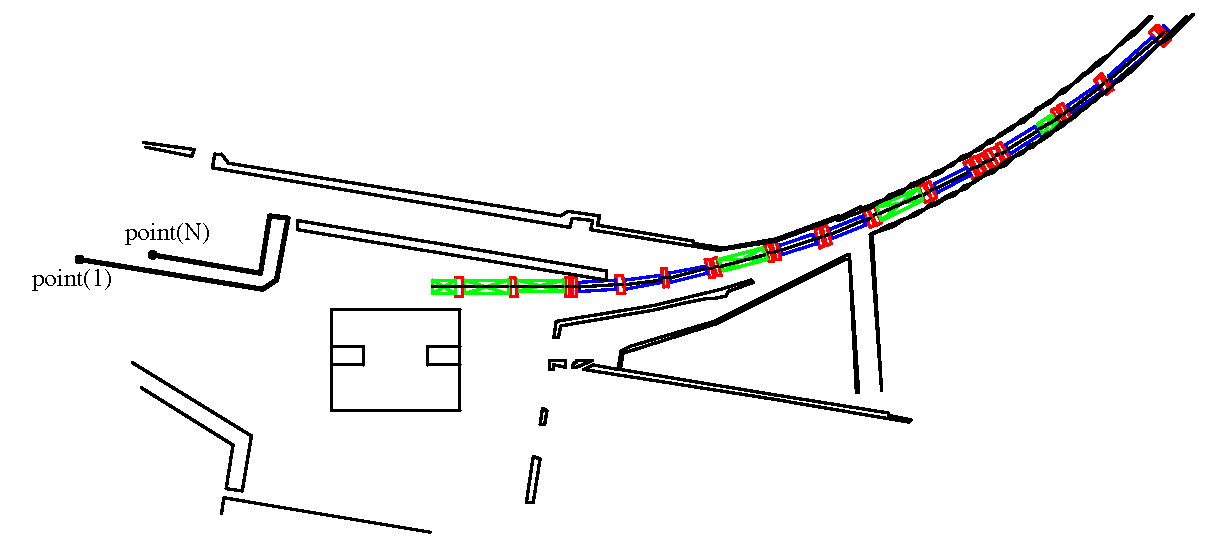
\includegraphics[width=5in]{building-wall.pdf}
  \caption[Floor plot showing the walls of the building]
{Floor plot showing the walls of the building (along with a section
of a recirculation arc). Defining building walls can be useful for
such things as floor plots and designing a machine to fit in an
existing building.}
  \label{f:building.wall}
\end{figure}

A two dimensional outline of the building containing the machine under
simulation may be defined in \tao. This may be useful when drawing
floor plans of the machine (\sref{s:floor.plan}) or to design a
machine to fit within an existing building by optimizing
(\sref{c:opti}) the position of the machine to be within the
building's walls.

The walls of a building are defined by a set of ``sections'' which are
just curves that mark the wall boundaries. One such section is
highlighted in Figure~\ref{f:building.wall} starting at the point
marked ``point(1)'' and ending at the point marked ``point(N)''. Each
section is defined by a set of points which are connected together using
straight lines or circular arcs.

The name of the file containing the building wall definition is given
by the \vn{building_wall_file} variable in the \vn{tao_start} namelist
(\sref{s:init.global}). This file will contain a number of
\vn{building_wall_section} namelists. Each \vn{building_wall_section}
namelist defines a single wall section. The syntax of this namelist is
\begin{example}
  &building_wall_section
    \{constraint = <type>\}
    point(1) = <z1>, <x1>
    point(2) = <z2>, <x2>, \{<r2>\}
    point(3) = <z3>, <x3>, \{<r3>\}
    ... etc ...
    point(N) = <zN>, <xN>, \{<rN>\}
  /
\end{example}
The global coordinate system in \bmad (see the \bmad manual) defines
the $(Z, X)$ plane as being horizontal.  [Note: $(Z, X)$ is used
instead of $(X, Z)$ since $(Z, X, Y)$ forms a right handed coordinate
system.] The points that define a wall section are specified in this
coordinate system.  In the \vn{building_wall_section} namelist, the
$(Z, X)$ position of each point defining a wall section is given along
with an optional radius $r$. If a non-zero radius is given for point
$j$, then the segment between point $j-1$ and $j$ is a circular arc of
the given radius. If no radius is given, or if it is zero, the segment
is a straight line. A radius for the first point, number 1, cannot be
specified since this does not make sense. Additionally, a radius must
be at least half the distance between the two points that define the
end points of the arc.

In general, given two end points and a radius, there are four possible
arcs that can be drawn. The arc chosen follows the following convention:
\begin{enumerate}
\item
The angle subtended by the arc is 180 degrees or less.
\item
If the radius for the arc from $j-1$ to $j$ is positive, the arc
curves in a clockwise manner. If the radius is negative, the arc
curves counterclockwise. This convention mimics the convention used
for \vn{rbend} and \vn{sbend} elements.
\end{enumerate}
To define a wall that is circular, use three points with two 180
degree arcs in between.

When designing a machine to fit within the walls of a building, the
\vn{constraint} variable of the namelist is used to designate whether
the given wall section is on the $+x$ side of the machine or the $-x$
side. Here $x$ is the local reference frame transverse coordinate. See
the write up of the \vn{wall.right_side} and \vn{wall.left_side} constraints in
\sref{s:data.types} for more details. Possible values for
\vn{constraint} are:
\begin{example}
  "right_side"  ! Section is to be used with wall.x+ constraints
  "left_side"   ! Section is to be used with wall.x- constraints
  "none"        ! Default. Section is ignored in any constraint calculation.
\end{example}

Example:
\begin{example}
  &building_wall_section
    constraint = "left_side"   
    point(1) =  23.2837,    8.2842
    point(2) = -10.9703,   13.8712, 107.345
    point(3) = -10.8229,   14.7737
  /
\end{example}
In this example, point 1 is at $(Z, X) = (23.2837, 8.2842)$, the
segment between points 1 and 2 is an arc with a radius of 107.345
meters, and the segment between points 2 and 3 is a straight
line. Also this wall section is to be used when evaluating any
\vn{wall.x+} constraint.

Note: To position a machine in the global coordinate system, the
starting point and starting orientation can be adjusted using
\vn{beginning[...]} statements as explained in the \bmad manual.

%-----------------------------------------------------------------
\section{Initializing Plotting}\index{plotting initializing}
\label{s:init.plot} 

\subsection{Plot Window}
\label{s:plot.page}
\index{initialization!plotting!plot window}

\begin{figure}
  \centering
  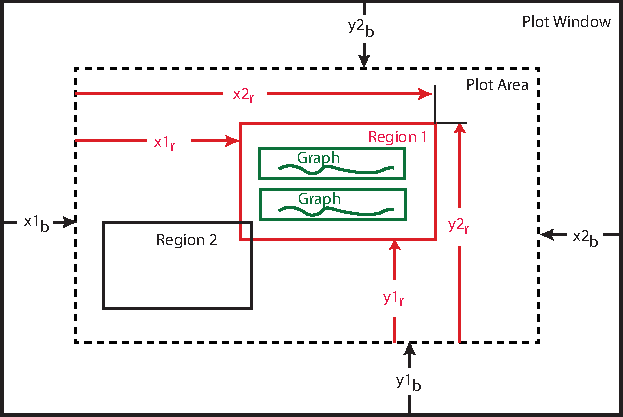
\includegraphics{plot-page.pdf}
  \caption{Regions define where on the plot page plots are placed.}
  \label{f:plot.page}
\end{figure}

Plotting is defined by an initialization file whose name is defined
by the \vn{tao_start} namelist (\sref{s:init.global}).
The first namelist block in the file has a block
name of \vn{tao_plot_page}. This block sets the size of the plot
window (also called the plot page) and defines the ``regions'' where
plots go. The syntax of this block is:
\index{tao_plot_page}    
\index{plot_page!n_curve_pts}
\index{plot_page!size}
\index{plot_page!border}
\index{plot_page%floor_plan_rotation}
\index{plot_page%floor_plan_view}
\index{plot_page!text_height}
\index{plot_page!title}
\index{region!name}
\index{region!location}
\index{place}
\begin{example}
  &tao_plot_page
    plot_page%plot_display_type      = <string>  ! Display type: 'X' or 'TK'
    plot_page%size                   = <x_size>, <y_size>         ! size in POINTS 
    plot_page%border                 = <b_x1>, <b_x2>, <b_y1>, <b_y2>, "<units>"
    plot_page%text_height            = <num>    ! height in POINTS. Def = 12
    plot_page%main_title_text_scale  = <num>    ! Relative to text_height. Def = 1.3
    plot_page%graph_title_text_scale = <num>    ! Relative to text_height. Def = 1.1
    plot_page%axis_number_text_scale = <num>    ! Relative to text_height. Def = 0.9
    plot_page%axis_label_text_scale  = <num>    ! Relative to text_height. Def = 1.0
    plot_page%legend_text_scale      = <num>    ! Relative to text_height. Def = 0.8
    plot_page%floor_plan_rotation    = <num>    ! Rotation of floor plan plot: 1.0 -> 360^deg 
    plot_page%floor_plan_view        = <string> ! Either: 'xz' (default), 'xy', or 'yz'
    plot_page%key_table_text_scale   = <num>    ! Relative to text_height. Def = 0.9
    plot_page%title(i)               = <string>, {<x>, <y>, "<units>", "<justify>"}
    plot_page%n_curve_pts            = <num>    ! Num points used to construct a 
                                                !   smooth curve. Default = 401
    plot_page%box_plots              = <T/F>    ! For debugging. Default = F.
    include_default_plots            = <T/F>    ! Include default plot templates? Def = F.
    region(i) = "<region_name>" <l_x1>, <l_x2>, <l_y1>, <l_y2>  ! % plot area
    place(i)  = "<region_name>", "<template_name>"
    default_plot%...                            ! See below.
    default_graph%...                           ! See below. 
  /
\end{example}
For example:
\begin{example}
  &tao_plot_page
    plot_page%plot_display_type = "X"        ! X11 window.  "TK" is alternative.
    plot_page%size        = 700, 800         ! Points
    plot_page%border      = 0, 0, 0, 50, "POINTS"  
    plot_page%text_height = 12.0
    plot_page%title(1)    = "CESR Lattice", 0.5, 0.996, "%PAGE", "CC"
    region(1) = "top"    0.0, 1.0, 0.5, 1.0
    region(2) = "bottom" 0.0, 1.0, 0.0, 0.5
    place(1)  = "top",    "orbit"
    place(2)  = "bottom", "phase"
    default_plot%x%min = 100
    default_plot%x%max = 200
  /
\end{example}

\vn{plot_page%size} sets the horizontal and vertical size of the plot
window in \vn{POINTS} units (72 points = 1 inch. Roughly 1 point = 1
pixel). 

\vn{plot_page%text_height} sets the overall height of the text that is
drawn. Relative to this, various parameters can be used to scale
individual types of text:
\begin{example}
  plot_page%main_title_text_scale  = 1.3 ! Main title height. 
  plot_page%graph_title_text_scale = 1.1 ! Graph title height.
  plot_page%axis_number_text_scale = 0.9 ! Axis number height
  plot_page%axis_label_text_scale  = 1.0 ! Axis label height.
  plot_page%key_table_text_scale   = 0.8 ! Key Table text (\sref{s:key.table}).
  plot_page%legend_text_scale      = 0.9 ! Lat Layout or floor plan text.
\end{example}
The default values for these scales are given above.

The \vn{plot_page%plot_display_type} component sets the type of plot display
window used. possibilities are:
\begin{example}
  "X"      X11 window   
  "TK"     tk window   
\end{example}

\vn{plot_page%border} sets a border around the edges of the
window. As shown in Figure~\ref{f:plot.page} \vn{b_x1}, \vn{b_x2} are
the right and left border widths and \vn{b_y1} and \vn{b_y2} are the
bottom and top border widths respectively.  The rectangle within this
border is called the plot area.

\vn{plot_page%title(i)} set the page title. There are two title areas 
(i = 1,2). If only the title string is given then the other variables 
are set to the defaults \vn{x} = 0.5, \vn{y} = 0.995, \vn{justify} = 
"CC" and \vn{units} = "%PAGE". See the quickplot documentation for 
the \vn{justify} variable syntax.

The plot area is divided up into rectangular regions where plots may
be placed (what defines a plot is discussed below).  \vn{region(i)} is
an array of five elements that defines the i\Th region. The first
element of this array is the name of the region. This name may not
contain a dot ``.''.  The second and third elements of the array,
\vn{l_x1}, and \vn{l_x2}, define the location of the left and right
edges of the region as a fraction of the plot area width starting from
the left edge of the plot area.  The final elements of the
\vn{region(i)} array, \vn{l_y1} and \vn{l_y2}.  define the location of
the bottom and top edges of the region as a fraction of the height of
the plot area with respect to the plot area's bottom edge. Thus, in
the above example, region 1 extends from the left border of the plot
area (\vn{region(1)%l_x1} = 0) to the right border
(\vn{region(1)%l_x2} = 0) and vertically from the center
(\vn{region(1)%l_y1} = 0.5) to the top edge (\vn{region(1)%l_x2} =
1.0). Regions may overlap any one can define as many regions as one
likes.

\vn{place(i)} determines the initial placement of plots.

\vn{default_plot} sets the defaults for any \vn{plot}s
defined in the \vn{tao_template_plot} namelists
(\sref{s:template}). Similarly, \vn{default_graph} sets defaults for the
\vn{graph} structure defined in the \vn{tao_template_graph} namelist
(\sref{s:template}). In the example above, the default x-axis min and
max are set to 100 and 200 respectively.

If \vn{include_default_plots} is set to \vn{True}, the collection of
default template plots (\sref{s:template}) that \tao uses by default
when no template plots are defined are used along with the template
plots defined in the plotting file.

%-----------------------------------------------------------------
\subsection{Plot Templates}
\label{s:template}
\index{plot templates}

As shown in Figure~\ref{f:plot}, a ``plot'' is made up of a collection
of ``graphs'' and a graph consists of axes plus a set of ``curves''.
In the \vn{tao_plot.init} file there needs to be defined a set of
``template plots''. A template plot specifies the layout of a plot:
How the graphs are placed within a plot, what curves are associated
with what graphs, etc. When running \tao, the information in a
template plot may then be transferred to a region using the \vn{place}
command and this will produce a visible plot.

Template plots are defined using namelists with a name of
\vn{tao_template_graph}. The general syntax is:
\index{tao_template_plot}
\index{plot!name}
\index{plot!x}
\index{plot!x_axis_type}
\index{plot!ix_universe}
\index{plot!n_graph}
\index{plot!autoscale_gang_x}
\index{plot!autoscale_gang_y}
\index{plot!autoscale_x}
\index{plot!autoscale_y}
\begin{example}
  &tao_template_plot
    plot%name        = "<plot_name>"
    plot%x           = <qp_axis_struct>
    plot%x_axis_type = "<x_axis_type>"   ! "index", "ele_index" "s", "lat", or "var". 
                                         ! Default is "index".
    plot%ix_universe = <number>          ! used for lat_layout plots
    plot%n_graph     = <n_graphs>
    plot%autoscale_gang_x = <logical>    ! Default: True.
    plot%autoscale_gang_y = <logical>    ! Default: True.
    plot%autoscale_x = <logical>         ! Default: False.
    plot%autoscale_y = <logical>         ! Default: False.
    default_graph%...                    ! See below
  /
\end{example}
For example:
\begin{example}
  &tao_template_plot
    plot%name                = "orbit"
    plot%x%min               =   0
    plot%x%max               = 100
    plot%x%major_div_nominal = 10
    plot%x%label             = "Index"
    plot%n_graph             = 2
    default_graph%y%max      = 10
  /
\end{example}

\vn{default_graph} sets defaults for the \vn{graph} structure defined
in the \vn{tao_template_graph} namelist (\sref{s:template}). This
overrides \vn{default_graph} settings made in the
\vn{tao_template_plot} namelist (\sref{s:init.plot}) but only for
graphs associated with the \vn{tao_template_plot} the
\vn{default_graph} is defined in.

\vn{plot%x} sets the properties of the horizontal axis. For more
information see the \vn{Quick Plot} documentation on the
\vn{qp_axis_struct} in the Bmad manual. The major components are
\index{qp_axis_struct!min}
\index{qp_axis_struct!max}
\index{qp_axis_struct!major_div_nominal}
\index{qp_axis_struct!major_div}
\index{qp_axis_struct!minor_div}
\index{qp_axis_struct!label}
\begin{example}
  min        ! Left edge value.
  max        ! Right edge value.
  major_div  ! Number of major divisions. 
             !  Number of major tick marks is one less.
  major_div_nominal ! Nominal number of major divisions
  minor_div  ! Number of minor divisions. 0 = auto choose.
  label      ! Axis label.
\end{example}
If \vn{min} and \vn{max} are absent, then \tao will autoscale the
axis.  If it is desired to have differing scales for different graphs,
the \vn{graph%x} component can be used (see below).

Both \vn{major_div} and \vn{major_div_nominal} set the number of major
divisions in the plot. The difference between the two is that with
\vn{major_div} the number of major divisions is fixed at the set value
and with \vn{major_div_nominal} the number of major divisions can vary
from the set value when \tao scales a graph. If
\vn{major_div_nominal} is set, this will override any setting of
\vn{major_div}. If neither \vn{major_div} nor \vn{major_div_nominal}
is set, a value will be chosen for \vn{major_div_nominal} by \tao. If
you are unsure which to set, it is recommended that
\vn{major_div_nominal} be used.

Plots with \vn{plot%autoscale_x} and/or \vn{plot%autoscale_y}
logicals, set to true will automatically rescale after any
calculation. The \vn{plot%autoscale_gang_x} and
\vn{plot%autoscale_gang_y} components set how the \vn{x_scale}
(\sref{s:x.scale}) and \vn{scale} (\sref{s:scale}) commands behave
when autoscaling entire plots. See these individual commands for more
details.

\vn{plot%name} is the name that is used with \tao commands to identify
the plot. It is important that this name not contain any blank spaces since
\tao uses this fact in parsing the command line. 

\vn{plot%x_axis_type} sets what is plotted along the
\vn{x_axis}. Possibilities are:
\index{index}
\index{ele_index}
\index{s}
\begin{example}
    "index"      ! Data Index
    "ele_index"  ! Element lattice number index
    "s"          ! Longitudinal position in the lattice.
    "data"       ! From a data array
    "lat"        ! Lattice variable. See \sref{s:plot.var}.
    "var"        ! Tao variable value. See \sref{s:plot.var}.

\end{example}
The \vn{ele_index} switch is used when plotting data arrays. In this
case the \vn{index} switch refers to the index of the data array and
\vn{ele_index} refers to the index of the lattice element that the
datum was evaluated at.

\vn{n_graph} sets the number of graphs associated with the plot and
each one needs a \vn{tao_template_graph} namelist to define it. These
namelists should be placed directly after their respective
\vn{tao_template_graph} namelists. The general format of the
\vn{tao_template_graph} namelist is:
\index{tao_template_graph}\index{graph!y}\index{curve!name}
\index{graph_index}\index{graph}\index{graph!name}\index{curve}
\index{graph!type}\index{graph!box}\index{graph!title}\index{graph!margin}
\index{graph!y2}\index{graph!n_curve}\index{graph!clip}\index{graph!component}
\index{graph%symbol_size_scale}
\index{curve!data_type}\index{curve!data_source}
\index{curve!x_axis_units_factor}\index{curve!y_axis_units_factor}
\index{curve!use_y2}\index{curve!line}\index{curve!ele_ref_name}
\index{curve!draw_line}\index{curve!draw_symbols}\index{curve!ix_universe}
\index{curve!symbol}\index{curve!symbol_every}\index{curve!convert}
\index{curve!ix_bunch}\index{curve!ix_ele_ref}\index{curve!data_type_x}
\begin{example}
  &tao_template_graph
    graph_index            = <number>
    graph%name             = "<string>"       ! Default is  "g<n>" <n> = graph_index. 
    graph%type             = "<string>"       ! "data", "floor_plan", etc.
    graph%box              = <ix>, <iy>, <ix_tot>, <iy_tot>
    graph%title            = "<string>"       ! Title above the graph.
    graph%margin           =  <ix1>, <ix2>, <iy1>, <iy2>, "<Units>"
    graph%scale_margin     =  <ix1>, <ix2>, <iy1>, <iy2>, "<Units>"
    graph%x                = <qp_axis_struct> ! Horizontal axis.
    graph%y                = <qp_axis_struct> ! Left axis.
    graph%y2               = <qp_axis_struct> ! Right axis.
    graph%clip             = <logical>        ! Clip curves at boundary? Default = T
    graph%draw_axes        = <logical>        ! Default = T
    graph%draw_grid        = <logical>        ! Default = T
    graph%component        = "<string>"       ! Eg: "model - design"
    graph%symbol_size_scale      = <real>     ! Phase_space plots symbol scale factor
    graph%correct_xy_distortion  = <logical>  ! For Floor Plan plots: Default = F
    graph%draw_only_good_user_data_or_vars    ! Veto data or variables with good_user = F?
                                 = <logical>  !   Default = T.
    graph%x_axis_scale_factor    = <factor>   ! Scale the x-axis by this.
    graph%n_curve                = <number>   ! number of curves
    curve(i)%name                = "<string>" ! Default is "c<i>", <i> = curve num.
    curve(i)%data_source         = "<string>" ! Source for the data curve points
    curve(i)%data_type_x         = "<string>" ! Used with plot%x_axis_type = "data" or "var".
    curve(i)%data_type           = "<string>" ! Default = plot%name.graph%name
    curve(i)%data_index          = "<string>" ! Index number for data points.
    curve(i)%legend_text         = "<string>" ! Text for curve legend. 
                                              !   Default is the data_type.
    curve(i)%y_axis_scale_factor = <factor>   ! Scale the y-axis by this.
    curve(i)%use_y2              = <logical>  ! Use left-axis scale?
    curve(i)%draw_line           = <logical>  ! Connect data with lines?
    curve(i)%draw_symbols        = <logical>  ! Draw data symbols?
    curve(i)%draw_symbol_index   = <logical>  ! Print index number next to the data symbol?
    curve(i)%ix_universe         = <number>   ! Default = -1 => Use viewed universe
    curve(i)%ix_branch           = <number>   ! Default = 0  => Use main lattice.  
    curve(i)%ix_bunch            = <integer>  ! Bunch index. Default = 0 (all bunches).
    curve(i)%line        = <qp_line_struct>   ! Line spec (color, width, etc.)
    curve(i)%symbol      = <qp_symbol_struct> ! Symbol spec (color size, etc.)
    curve(i)%symbol_every     = <integer>     ! Plot symbol every # datums
    curve(i)%ele_ref_name     = "<string>"    ! Name of reference element.
    curve(i)%ix_ele_ref       = <num>         ! Index number of reference element.
    curve(i)%smooth_line_calc = <Logical>     ! Calc data between symbol points? 
  /
\end{example}
For example:
\begin{example}
  &tao_template_graph
    graph_index               = 1
    graph%name                = "x"
    graph%type                = "data"
    graph%box                 = 1, 1, 1, 2
    graph%title               = "Horizontal Orbit (mm)"
    graph%margin              =  60, 200, 30, 30, "POINTS"
    graph%y%label             = "X"
    graph%y%max               =  4
    graph%y%min               = -4
    graph%y%major_div_nominal = 4
    graph%n_curve             = 1
    graph%component           = "model - design"
    curve(1)%data_source      = "dat"
    curve(1)%data_type        = "orbit.x"
    curve(1)%units_factor     = 1000
    curve(1)%use_y2           = F
  /
\end{example}

\vn{graph%title} is the string just above the graph. The full string
will also include information about what is being plotted and the
horizontal axis type. To fully suppress the title leave it blank.

If there are multiple curves drawn with a graph then a curve legend
showing what lines are associated with what data will be drawn. The
default is to draw this legend in the upper left hand corner of the
graph. By default, the \vn{data_type} of each curve will be used as
the text for that curve's line in the legend.  This default can be
changed by setting a curve's \vn{curve%legend_tex}.

\vn{graph%name} and \vn{curve%name} define names to be used with
commands. The default names are just the letter \vn{g} or \vn{c} with
the index of the graph or curve. Thus, in the example above, the name
of the curve defaults to \vn{c1} and it would be referred to as
\vn{orbit.x.c1}.  It is important that these names do not contain any
blank spaces since \tao uses this fact in parsing the command line.

\vn{graph%box} sets the layout of the box which the \vn{graph} is
placed in. For a definition of what a box is see the Quick Plot
documentation in the \bmad reference manual. In the above example the
graph divides the region into two vertically stacked boxes and places
itself into the bottom one. 

\vn{graph%margin} sets the margin between the \vn{graph} and the \vn{box}
it is drawn in.

\vn{graph%scale_margin} is used to set the minimum space between what
is being drawn and the edges of the \vn{graph} when a \vn{scale},
\vn{x_scale}, or a \vn{xy_scale} command is issued. Normally this
is zero but is useful for \vn{floor plan} drawings.

\vn{graph%type} is the type of graph. \tao knows about the
following types:
\index{data}\index{lat_layout}\index{key_table}\index{phase_space}
\index{floor_plan}\index{beam_chamber_wall}
\begin{example}
  "data"               ! Data and/or variable plots (default) (\sref{s:plot.data}).
  "floor_plan"         ! A 2-dimensional birds-eye view of the machine (\sref{s:floor.plan}).
  "histogram"          ! Histogram of plot (\sref{s:histogram}).
  "key_table"          ! Key binding table for single mode (\sref{s:key.table}).
  "lat_layout"         ! Schematic showing placement of the lattice elements (\sref{s:lat.layout}).
  "phase_space"        ! Phase space plots (\sref{s:phase.space}).
\end{example}

With \vn{graph%type} set to \vn{"beam_chamber_wall"}
(\sref{s:beam.wall.draw}), the beam chamber wall is drawn if it has
been defined in the \bmad lattice file.

With \vn{graph%type} set to \vn{"data"} (\sref{s:plot.data}), data such
as orbits and/or variable values such as quadrupole strengths are
plotted. Here ``data'' can be data from a defined data structure
(\sref{c:data}) or computed directly from the lattice, beam tracking,
etc. A \vn{"data"} graph type will contain a number of \vn{curves} and
multiple data and variable curves can be drawn in one graph.

With \vn{graph%type} set to \vn{floor_plan} (\sref{s:floor.plan}), the
two dimensional layout of the machine is drawn.

With \vn{graph%type} set to \vn{histogram} (\sref{s:histogram}), such
things such as beam densities can be histogrammed.

With \vn{graph%type} set to \vn{"key_table"} (\sref{s:key.table}), the
key bindings for use in single mode (\sref{s:key.bind}) are displayed.
Note: The \vn{"key_table"} graph type does not have any associated
\vn{curve}s.

With \vn{graph%type} set to \vn{lat_layout} (\sref{s:lat.layout}), the
elements of the lattice are symbolical drawn in a one dimensional
line as a function of the longitudinal distance along the machine
centerline.

With \vn{graph%type} set to \vn{phase_space} (\sref{s:phase.space}),
phase space plots are produced.

%-----------------------------------------------------------------
\subsection{Data and Variable plotting}
\label{s:plot.data}

A \vn{graph} (\sref{s:template}), with \vn{graph%type} equal to
\vn{"data"}, is used to draw ``data'' such as orbits and/or variable
values such as quadrupole strengths. A data \vn{graph} will have a
number of associated \vn{curve}s with each curve defining a particular
data type to plot. 

The data values will depend upon where the data
comes from. This is determined, in part, by the setting of
\vn{graph%component}. \vn{graph%component} may be one of:
\index{model}\index{design}\index{base}\index{meas}\index{ref}
\begin{example}
  "model"             ! model values. Default.
  "design"            ! design values.
  "base"              ! Base values
  "meas"              ! data values.
  "ref"               ! reference data values.
  "beam_chamber_wall" ! Beam chamber wall
\end{example}
The default, if \vn{graph%component} is not specified, is to use
\vn{"model"}. Additionally, \vn{graph%component} may be set to plot a
linear combination of the above. For example:
\begin{example}
  graph%component = "model - design"
\end{example}
This will plot the difference between the \vn{model} and \vn{design}
values.

\index{dat}\index{var}\index{calculation}
\index{curve!data_source}
The \vn{curve} structure is used to define the data that is plotted
in each graph. \vn{curve%data_source} is the type of information for
the source of the data points. \vn{curve%data_source} must be one of:
\begin{example}
  "dat"               ! A d1_data array is the source of the curve points.
  "var"               ! A v1_var array is the source of the curve points.
  "lat" (Default)     ! The curve points are computed directly from the lattice.
  "beam"              ! The curve points are computed tracking a beam of particles.
  "multi_turn_orbit"  ! Computation is from multi-turn tracking. 
\end{example}
The default for \vn{curve%data_source} is \vn{"lat"}. With
\vn{curve%data_source} set to \vn{dat}, the values of the curve
points come from the \vn{d1_data} array structure named by
\vn{curve%data_type}. Thus in the above example the curve point values
are obtained from \vn{orbit.x} data. To be valid the data structure
named by \vn{curve%data_type} must be set up in an initialization
file. If not given, the default \vn{curve%data_type} is
\begin{example}
  <plot%name>.<graph%name>
\end{example}
If \vn{curve%data_source} is set to \vn{var}, the values of the
curve points come from a \vn{v1_var} array structure. If it is set to
\vn{lat} the curve data points are calculated from the lattice
without regard to any data structures. \vn{curve%data_source} can be
set to \vn{beam} when tracking beams of particles. In this case, the
curve points are calculated from the tracking. With \vn{beam}, the
particular bunch that the data is extracted from can be specified via
\vn{curve%ix_bunch}. The default is \vn{0} which combines all the
bunches of the beam for the calculation.

Example: With \vn{curve%data_type} set to \vn{beta.x}, the setting of
\vn{curve%data_source} to \vn{lat} gives the beta as calculated
from the lattice and \vn{beam} gives the beta as calculated from the
shape of the beam.

\vn{curve%draw_symbols} determines whether a symbol is drawn at the
data points. The size, shape and color of the symbols is determined by
\vn{curve%symbol}. A given symbol point that is drawn has three
numbers attached to it: The $(x, y)$ position on the graph and an
index number to help identify it. The index number of a particular
symbol is the index of the datum or variable corresponding the symbol
in the \vn{d1_data} or \vn{v1_var} array. These three numbers can be
printed using the \vn{show curve -symbol} command (\sref{s:show}).
\vn{curve%draw_symbol_index} determines whether the index number is
printed besides the symbol. Use the \vn{set curve} command
(\sref{s:set}) to toggle the drawing of symbols. The default value for
\vn{curve%draw_symbol} is False if \vn{plot%x_axis_type} is \vn{"s"}
and True otherwise. The default\vn{curve%draw_symbol_index} is always
False.

\vn{curve%draw_line} determines whether a curve is drawn through the
data point symbols. The thickness, style (solid, dashed, etc.), and
color of the line can be controlled by setting \vn{curve%line}. If
\vn{plot%x_axis_type} is \vn{"s"}, and \vn{graph%component} does not
contain \vn{"meas"} or \vn{"ref"}, \tao will attempt to calculate
intermediate values in order to draw a smooth, accurate curve is
drawn. Occasionally, this process is too slow or not desired for other
reasons so setting \vn{curve%smooth_line_calc} to False will prevent
this calculation and the curve will be drawn as a series of lines
connecting the symbols. The default of \vn{curve%smooth_line_calc} is
True. Use the \vn{set curve} command (\sref{s:set}) to toggle the
drawing of lines.

The \vn{graph%draw_only_good_user_data_or_vars} switch determines
whether datums (\sref{s:init.data}) or variables (\sref{s:init.var})
with a \vn{good_user} component set to \vn{False} are drawn. The
default is to not draw them which means that data or variables not
used in an optimization are not drawn. 

A graph has two vertical axes. The one on the left is called \vn{"y"}
and the one on the right is called \vn{"y2"}. For example,
\vn{graph%y%label} sets the axis label for the \vn{y} axis and
\vn{graph%y2%label} sets the axis label for the \vn{y2} axis. Normally
there is only one vertical scale for a graph and this is associated
with the \vn{y} axis. However, if any curve of a given graph has
\vn{curve%use_y2} set to \vn{True} then the \vn{y2} axis will have an
independent second scale. In this case, the \vn{y2} axis numbers will
be drawn. Notice that simply giving the \vn{y2} axis a label does {\em
not} make the \vn{y2} axis scale independent of the \vn{y} axis scale.

Typically, a graph's horizontal scale is set by the \vn{plot%x}
component. If it is desired to have differing scales for different
graphs, the \vn{graph%x} component can be used.

%-----------------------------------------------------------------
\subsection{Graphing a Data Slice}\index{plot!data slice}
\label{s:graph.data.slice}

The standard data graph, as presented in the previous subsection,
plots data from a given \vn{d1_data} array. It is also possible to
graph data that has been ``sliced'' in other ways. For example,
suppose a number of universes have been established, with each
universe representing the same machine but with different steerings
powered. If in each universe an \vn{orbit} \vn{d2_data} structure has
been defined, an example of a data slice is the collection of
points (x, y) where:
\begin{example}
  (x, y) = (<n>@orbit.x[23], <n>@orbit.y[23]),   <n> = 1, ..., n_universe
\end{example}
When defining a template for graphing a data slice, the
plot%x_axis_type is set to \vn{"data"}, and the \vn{graph%type} must
be set to \vn{"data"}, the \vn{curve(:)%data_source} must be set to
\vn{"dat"} and the \vn{curve(:)%data_type_x} and
\vn{curve%data_type} are used to define the x and y axes respectively.
In the strings given by \vn{<curve%data_type_x} or
\vn{<curve%data_type}, all substrings that look like \vn{\#ref} are
eliminated and the string given by \vn{curve%ele_ref_name} is
substituted in its place.  Similarly, a \vn{\#comp} string is used as a
place holder for the \vn{graph%component} Example:
\begin{example}
  &tao_template_plot
    plot%name = "at_bpm"
    plot%x%label = "x"
    plot%x_axis_type = "data"
    plot%n_graph = 1
  /

  &tao_template_graph
    graph_index = 1
    graph%title = "Orbit at BPM"
    graph%y%label = "y"
    graph%component = "meas - ref"
    graph%type = "data"
    graph%n_curve = 1
    graph%x_axis_scale_factor = 1000
    curve(1)%data_source = "dat"
    curve(1)%data_type_x = "[2:57]@orbit.x[#ref]|#comp"
    curve(1)%data_type   = "[2:57]@orbit.y[#ref]|#comp"
    curve(1)%data_index  = "[2:57]@orbit.y[#ref]|ix_uni"
    curve(1)%y_axis_scale_factor = 1000
    curve(1)%ele_ref_name = "23"
    curve(1)%draw_line = F
  /
\end{example}
In this example, \vn{curve(1)%data_type_x} expands to
\vn{"[2:57]@orbit.x[23]|meas-ref"}. That is, the \vn{meas - ref}
values of \vn{orbit.x[23]} from universes 2 through 57 is used for the
x-axis.  Similarly, \vn{orbit.y[23]} is used for the y-axis. The
\vn{set} command (\sref{s:set}) can be used to change
\vn{curve%ele_ref_name} and \vn{graph%component} strings. 

\vn{curve%data_index} sets the index number for the symbol points
(\sref{s:template}). In the above example, \vn{curve%data_index} is
set to \vn{"[2:57]@orbit.y[\#ref]|ix_uni"}. The \vn{|ix_uni} component
will result in the symbol index number being the universe number.
Additionally, the component \vn{|ix_d1} can be used to specify the
index in the \vn{d1_data} array, and the component \vn{|ix_ele} can be
used to specify the lattice element index. Setting the symbol index
number is important when \vn{curve%draw_symbol_index} is set to True
so that the symbol index is drawn with the curve. Additionally, the
command \vn{show curve -symbol} (\sref{s:show}) will print the symbol
index number along with the $(x, y)$ coordinates of the symbols.

Arithmetic expressions (\sref{s:arithmetic.exp}) may be mixed with
explicit datum components in the specification of
\vn{curve(:)%data_type_x} and \vn{curve(:)%data_type}. Example:
\begin{example}
  curve(1)%data_type_x = "[#ref]@orbit.x|model"
  curve(1)%data_type   = "[#ref]@orbit.x|meas-ref"
  curve(1)%ele_ref_name = "3"
\end{example}
The plots the \vn{model} values of \vn{orbit.x} verses \vn{meas - ref}
of \vn{orbit.x} for the data in universe 3. Note: Whenever explicit
components are specified, the \vn{graph%component} settings are ignored for
that expression.

%-----------------------------------------------------------------
\subsection{Plotting With a Variable Value on the X-Axis}
\index{plot!plotting as a function of a variable}
\label{s:plot.var}

Data can be plotted as a function of a variable by setting
\vn{plot%x_axis_type} to \vn{"lat"} (for lattice variables) or
\vn{"var"} (for \tao variables) and setting \vn{curve(:)%data_type_x}
to the name of the variable. In this case, the \vn{curve(:)%data_type}
must evaluate to a single number.

Example:
\begin{example}
  &tao_template_plot
    plot%x_axis_type = "lat"
    ...
  /

  &tao_template_graph
    ...
    curve(1)%data_type_x = "beam_start[x]"  ! X-axis values.
    curve(1)%data_type   = "orbit.x[10]"    ! Y-axis values.
    ...
  /
\end{example}

Note: \tao treats the \vn{design} and \vn{base} lattices as static so
that varying a variable will not affect these lattices. Thus,
constructing a plot with \vn{graph%component} set to, for example,
\vn{"model - design"} will {\em not} produce a plot that is the
difference between varying a variable in both \vn{model} and
\vn{design} lattices. In the case where such a plot is desired, a
second universe needs to be established. In this case, one would set
\vn{curve(:)%data_type} to something like
\begin{example}
    curve(1)%data_type   = "1@orbit.x[10] - 2@orbit.x[10]"    
\end{example}
where the universe \#2 \vn{model} lattice would be setup to be equal
to the universe \#1 \vn{design} lattice.

%-----------------------------------------------------------------
\subsection{Drawing a Lattice Layout}
\index{lattice layout}
\label{s:lat.layout}

\begin{figure}
  \centering
  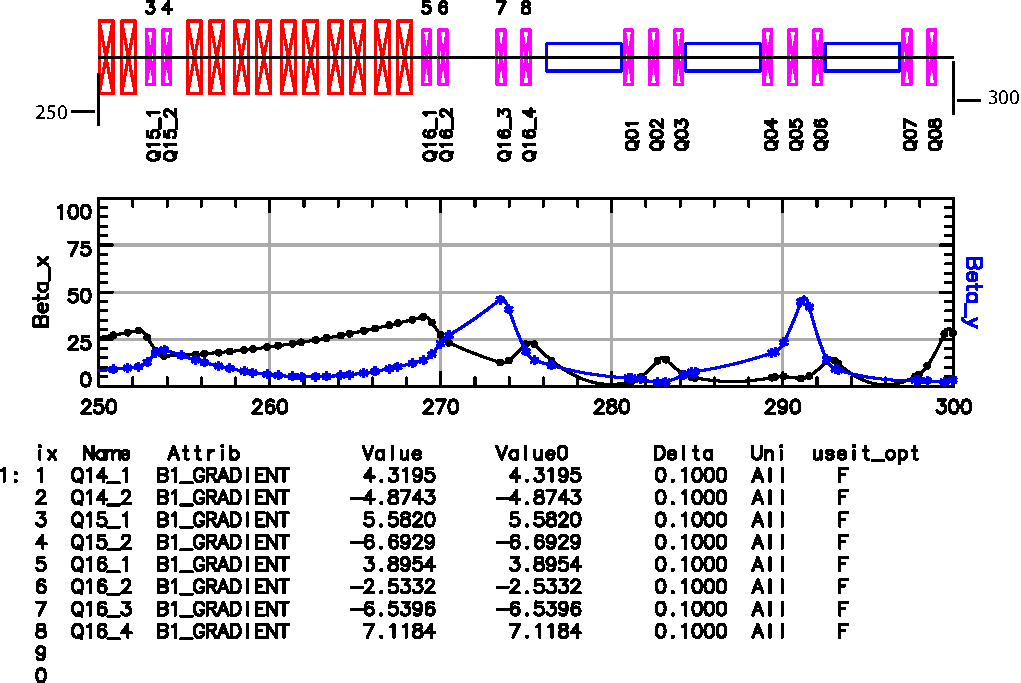
\includegraphics[width=5in]{layout-graph-table.pdf}
  \caption[Example lattice layout and data plots]
{A lattice layout plot (top) above a data plot (middle) 
which in turn is above a key table plot (bottom). The points on the
curves in the data plot mark the edges of the elements displayed in
the lattice layout. Elements that have attributes that are varied as
shown in the key table have the corresponding key table number printed
above the element's glyph in the lattice layout.}
  \label{f:layout.table}
\end{figure}

A lattice layout plot draws the lattice
along a straight line with colored rectangles representing the various elements.
An example is shown in Figure~\ref{f:layout.table}.
The \vn{tao_template_plot} needed to define a lattice layout looks like:
\index{tao_template_plot}\index{plot!name}
\index{plot!x!min}\index{plot!x!max}\index{plot!n_graph}
\index{tao_template_graph}\index{graph_index}\index{graph!name}
\index{graph!type}\index{graph!title}\index{graph!box}
\index{graph!ix_universe}\index{graph!margin}\index{graph!n_curve}
\begin{example}
  &tao_template_plot
    plot%name        = "<plot_name>"
    plot%x%min       = <number>
    plot%x%max       = <number>
    plot%n_graph     = <number>
    plot%x_axis_type = "s"
  /
  &tao_template_graph
    graph_index       = <number>
    graph%name        = <name>
    graph%type        = "lat_layout"
    graph%title       = "Layout Title"
    plot%box          = <ix>, <iy>, <ix_tot>, <iy_tot>
    graph%ix_universe = <integer> ! -1 => use currently viewed universe
    graph%ix_branch   = <integer> !  0 => use main lattice.
    graph%margin      = <ix1>, <ix2>, <iy1>, <iy2>, "<Units>"
    graph%y%min       = <real>    ! Default: -100
    graph%y%max       = <real>    ! Default:  100
  /
\end{example}
Example:
\begin{example}
  &tao_template_plot
    plot%name        = "layout"
    plot%x%min       =   0
    plot%x%max       = 100
    plot%n_graph     = 1
    plot%x_axis_type = "s"
  /

  &tao_template_graph
    graph_index       = 1
    graph%name        = "u1"
    graph%type        = "lat_layout"
    graph%box         = 1, 1, 1, 1
    graph%ix_universe = 1
    graph%margin      = 0.12, 0.12, 0.30, 0.06, "%BOX"
  /
\end{example}

Which elements are drawn is under user control and is defined 
using an \vn{lat_layout_drawing} namelist. See Section~\sref{s:layout.and.floor}
for more details.

The longitudinal distance markers at either end of the lattice layout can be 
suppressed by setting
\begin{example}
  graph%x%draw_numbers = F
\end{example}

%-----------------------------------------------------------------
\subsection{Drawing a Floor Plan}
\index{floor plan drawing}
\label{s:floor.plan}

\begin{figure}
  \centering
  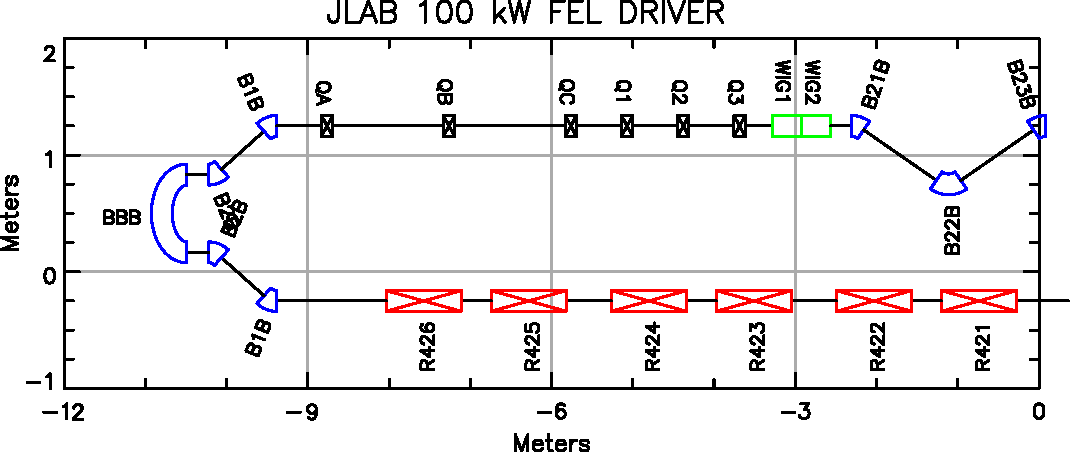
\includegraphics[width=5in]{floor-plan.pdf}
  \caption{Example Floor Plan drawing.}
  \label{f:floor.plan}
\end{figure}

A \vn{Floor Plan} drawing gives a display of the machine projected
onto the horizontal plane.  An example is shown in
Figure~\ref{f:floor.plan}. Like a \vn{Lattice Layout}
(\sref{s:lat.layout}), Elements are represented by colored rectangles
and which elements are drawn is determined by an
\vn{floor_plan_drawing} namelist (see~\sref{s:layout.and.floor}).

The placement of an element in the drawing is determined by the
element's coordinates in \vn{global reference system}.  See the Bmad
manual for more information on the \vn{global reference system}.  In
the \vn{global reference system}, the $(Z, X)$ plane is the horizontal
plane.  The conversion between the $(Z, X)$ coordinates of the
\vn{global reference system} and the $(x, y)$ coordinates of the floor
plan plot are:
\begin{example}
Global       Plot
  Z    <--->   x
  X    <--->   y
\end{example}
Drawing a plane other than the horizontal $(Z, X)$ plane can be set using
the \vn{plot_page%floor_plan_view} switch. Valid settings for this switch are
\begin{example}
  'xz'     ! Default
  'xy'
  'yz'
\end{example}
An overall rotation of the floor plan can be controlled by setting
\vn{plot_page%floor_plan_rotation} in the \vn{tao_plot_page} namelist. Example:
(\sref{s:init.plot})
\begin{example}
  &tao_plot_page
    plot_page%floor_plan_rotation = 0.5  ! Rotate 180 degress
  /
\end{example}


Alternatively, the global coordinates at the start of the lattice can
be defined in the lattice file and this can rotate the floor plan.
Unless there is an offset specified in the lattice file, a lattice
will start at $(x, y) = (0, 0)$. Assuming that the machine lies in the
horizontal plane with no negative bends, the reference orbit will
start out pointing in the negative $x$ direction and will circle
clockwise in the $(x, y)$ plane.

Example Floor Plan template:
\begin{example}
  &tao_template_plot
    plot%name = "floor"
    plot%x%min = -12  
    plot%x%max = 0    
    plot%x%major_div_nominal = 4
    plot%x%minor_div = 3
    plot%x%label = "Meters"
    plot%n_graph = 1
  /

  &tao_template_graph
    graph_index = 1
    graph%name = "1"
    graph%type = "floor_plan"
    graph%box = 1, 1, 1, 1
    graph%margin = 0.10, 0.10, 0.10, 0.10, "%BOX"
    graph%ix_universe = 1
    graph%y%label = "Meters"
    graph%y%max = 2  
    graph%y%min = -1 
    graph%correct_xy_distortion = T
  /
\end{example}
To prevent the drawing of the axes set \vn{graph%draw_axes} to False.
To prevent the drawing of a grid at the major division points set
\vn{graph%draw_grid} to False.

By default, the horizontal or vertical margins of the graph will be
increased so that the horizontal scale (meters per plotting inch) is
equal to the vertical scale.  If \vn{graph%correct_xy_distortion} is
set to \vn{False}, this scaling will not be done.

Note: The \vn{show ele -floor} command (\sref{s:show}) can be used to
view an element's global coordinates.

%-----------------------------------------------------------------
\subsection{Defining Shapes for Lat_layout and Floor_plan Drawings}
\index{lat_layout drawings}
\index{floor_plan drawings}
\label{s:layout.and.floor}

\vn{Floor plan} (\sref{s:floor.plan}) and \vn{lattice layout} drawings
use various shapes, sizes, and colors to represent lattice
elements. The association of a particular element with a given shape
is determined via two namelists: \vn{lat_layout_drawing} for the
lattice layout and \vn{floor_plan_drawing} for floor plan drawings.
Two different namelists are used since, for example, a size that is
good for a layout will not necessarily be good for a floor plan.

The namelist syntax is the same for both:
\begin{example}
  &lat_layout_drawing
    ele_shape(i) = "<name>" "<shape>" "<color>" "<v_size>" "<label>" <draw> 
  /

  &floor_plan_drawing
    ... same as lat_layout_drawing ...
  /
\end{example}
For Example:                 
\begin{example}
  &floor_plan_drawing
    !               name                    Shape     Color  V_Size   Label Draw?
    ele_shape(1) = "quadrupole::q*"         "box"     "red"     0.75     "name"  T    
    ele_shape(2) = "quadrupole::*"          "xbox"    "red"     0.75     "none" 
    ele_shape(3) = "sbend::*"               "box"     "blue"    0.37     "none"  F
    ele_shape(4) = "wiggler::*"             "xbox"    "green"   0.50     "name"
    ele_shape(5) = "var::quad_k1"           "circle"  "purple"  0.25     "name"
    ele_shape(6) = "dat::orbit.x|useit_opt" "x"       "orange"  0.25     "name"
    ele_shape(7) = "wall::building"         "-"       "black"    0       "-"
  /
\end{example}
A figure is drawn for each lattice element in the lattice that matches the
\vn{<name>} specification (\sref{s:ele.list.format}) of any \vn{ele_shape(:)}.
Thus, in the example above, \vn{ele_shape(1)} will match to all
quadrupoles whose name begins with ``q'' and \vn{ele_shape(2)} will
match all quadrupoles. If an element matches more than one shape the
first shape matched will be used. For a floor plan, for \vn{wiggler}s that have an
\vn{x_ray_line_len} attribute, The X-ray line will be drawn if an
\vn{ele_shape} for a \vn{photon_branch} is present.

Use the \vn{show plot -shape} command to see the defined shapes.  use
the \vn{set shape} command (\sref{s:set})) to set shape parameters on the
command line.

Data and variables can also be specified to be drawn by using a
\vn{name} beginning with \vn{dat::} for drawing data and \vn{var::}
for drawing variable locations. In the above example, it is assumed
that a \vn{quad_k1} variable array and a \vn{orbit.x} data array have
been setup. A circle will be drawn at each element under control of a
\vn{quad_k1} variable. For the \vn{orbit.x} data, an ``x'' will de
drawn where the data is being evaluated but only for datums whose
\vn{useit_opt} parameter is True.

For \vn{floor_plan} drawings, the building wall
(\sref{s:building.wall}) can be drawn by specifying an \vn{ele_sape}
whose name is \vn{"wall::building"}. For the building wall, the only
\vn{ele_shape} attribute that is relavent is the \vn{color}.

The \vn{<shape>} parameter is the shape of the figure
drawn. Valid Shapes are:
\index{box}\index{xbox}
\begin{example}
  "asym_var_box"    -- Like var_box but is not symmetric about the center line. 
  "box"             -- Rectangular box
  "bow_tie"         -- Bow-tie shape.
  "circle"          -- Circle centered at center of element.
  "diamond"         -- Diamond shape.
  "var_box"         -- Rectangular box with variable height. 
                        The box is symmetric about the center line.
  "x"               -- "X" centered at center of element
  "xbox"            -- Rectangular box with an x through it.
\end{example}

The width of a drawn shape is the width of the associated element. The
exception is the \vn{"x"} shape whose width is always the same as the
height determined by the \vn{<v_size>} setting.

\vn{<v_size>} is the vertical half height of the shape.  For
\vn{lat_layout} drawings, \vn{<v_size>} = 1.0 corresponds to full
scale if the default \vn{graph%y%min} = -1 and \vn{graph%y%max} = 1
are used. For \vn{var_height_box}, the height is proportional to the
element strength and here \vn{<v_size>} is the multiplier used to
scale from element strength to vertical height. For example, for a
quadrupole the height is proportional to the \vn{K1} focusing
strength. Not all lattice elements can be used with a
\vn{var_height_box}.

\vn{<color>} is the color of the shape. Good colors to use are:
\index{element shape!color}
\begin{example}
  "black"
  "blue"
  "cyan"
  "green"
  "magenta"
  "orange"
  "purple"
  "red"
  "yellow"
\end{example}

The \vn{<label>} indicates what type of label to print next to the corresponding
element glyph. Possibilities are:
\begin{example}
  name            -- The element name (default).
  none            -- No label is drawn.
  s               -- Draw longitudinal s position.
\end{example}
The default is \vn{"name"}

The \vn{<draw>} field determines if a shape is drawn or not. The
default is \vn{T}. This can be useful for toggling on and off the
drawing of shapes using the \vn{set shape} command (\sref{s:set}).

Note: There is an old, deprecated syntax where both the lattice layout
and floor plan drawings are specified via one \vn{element_shapes}
namelist.

%-----------------------------------------------------------------
\subsection{Drawing a Histogram}
\index{histogram drawing}
\label{s:histogram}

A \vn{historgram} drawing displays a histogram of phase space beam
density. Histogram plotting is associated with a \vn{graph} by setting
\vn{graph%type} equal to \vn{"histogram"}. The concepts here are
similar to \vn{phase space} plotting (\sref{s:phase.space}). Example
histogram template:
\begin{example}
  &tao_template_plot
    plot%name = "zphase"
    plot%x%min =   -10e-3
    plot%x%max = 10e-3
    plot%x%major_div_nominal = 4
    plot%x%label = "z"
    plot%n_graph = 1
  /

  &tao_template_graph
    graph_index = 1
    graph%name = "z"
    graph%type = "histogram"
    graph%box = 1, 1, 1, 1
    graph%title = "Z"
    graph%margin =  0.12, 0.12, 0.12, 0.12, "%BOX"
    graph%y%label = "Density"
    graph%y%max = 3
    graph%y%min = -3
    graph%y%major_div_nominal = 4
    graph%n_curve = 1
    graph%bin_width = 1e-4
    curve(1)%data_type = "z" 
    curve(1)%data_source = "beam"
    curve(1)%ele_ref_name = "BEGINNING"
  /
\end{example}

For a \vn{"histogram"} type graph, \vn{curve%data_type} determines
what coordinate is plotted along the x-axis.
Valid \vn{curve%data_type} values are:
\index{x}\index{px}\index{y}\index{py}\index{z}\index{pz}
\begin{example}
  "x"
  "px"
  "y"
  "py"
  "z"
  "pz"
  "intensity"       -- Photon total intensity 
  "intensity_x"     -- Photon intensity along x-axis 
  "intensity_y"     -- Photon intensity along y-axis
  "phase_x"         -- Photon phase along x-axis
  "phase_y"         -- Photon phase along y-axis
\end{example}
In this example above, the $x$-axis of the plot will correspond to the
$z$ phase space coordinate.

The \vn{graph%bin_width} establishes the width of the histogram bins.

\index{curve!ele_ref_name}\index{curve!ix_ele_ref}
To change the place in the lattice where the data for the
\vn{histogram} is evaluated, use the \vn{set curve ele_ref_name} or
\vn{set curve ix_ele_ref} commands.

If \vn{graph%type} is \vn{"histogram"} then \vn{curve%data_source} 
must be either:
\begin{example}
  "beam"
  "multi_turn_orbit"
\end{example} 
\vn{"beam"} indicates that the points of the histogram plot
will be obtained correspond to the positions of the particles within a
tracked beam. \vn{multi_turn_orbit"} is used for rings where a single
particle is tracked multiple turns and the position of this particle
is recorded each turn. In this case, a \vn{d2_data} structure must
have been set up to hold the turn--by--turn orbit. This \vn{d2_data}
structure must be called \vn{multi_turn_orbit} and must have
\vn{d1_data} data arrays for the histogram planes to be plotted. For
example, if the histogram plot is \vn{x} versus \vn{px}, then there
must be \vn{d1_data} arrays named \vn{"x"} and \vn{"px"}. The number
of turns is determined by the setting of \vn{ix_max_data} in the
\vn{tao_d1_data} namelist (\sref{s:init.data}).

%-----------------------------------------------------------------
\subsection{Drawing the Beam Chamber Wall}
\index{beam chamber wall}
\label{s:beam.wall.draw}

If a beam chamber wall has been defined in the lattice file, This wall
can be drawn in a \vn{curve} by setting \vn{curve%type} to
\vn{"beam_chamber_wall"}.

Beam chamber walls are drawn, like a \vn{lat_layout}, on a one
dimensional line as a function of longitudinal position along the
machine centerline.

Note: Use the command \vn{show ele -wall} to print information about the
beam chamber wall for a particular element.

%-----------------------------------------------------------------
\subsection{Drawing a Key Table}
\index{key table}
\label{s:key.table}

The \vn{key table} is explained more fully in
Section~\sref{s:key.bind}.  An example is shown in
Figure~\ref{f:layout.table}. A template to create a key table looks
like:
\begin{example}
  &tao_template_plot
    plot%name = "table" 
    plot%n_graph = 1
  /

  &tao_template_graph
    graph%type = "key_table" 
    graph_index = 1
    graph%n_curve = 0
  /
\end{example}

The number in the upper left corner, to the left of the first column, 
(\vn{1} in Fig.~\ref{f:layout.table})
shows the active \vn{key bank}. The columns in the Key Table are:
\begin{example}
  Ix         ! Key index.
  Name       ! Element name whose attribute is bound.
  Attrib     ! Name of the element attribute that is bound.
  Value      ! Current value of bound attribute.
  Value0     ! Initial value of bound attribute.
  Delta      ! Change in value when the appropriate key is pressed.
  Uni        ! Universe that contains the element.
  Opt        ! Shows if bound attribute is used in an optimization.
\end{example}

Note that in a \vn{Lattice Layout}, if a displayed element has a bound
attribute, then the key index number will be displayed just above the
element's glyph.

The \vn{key_table} is drawn with respect to the upper left hand corner
of the region in which it is placed.

%-----------------------------------------------------------------
\subsection{Phase Space Plotting}
\index{phase space plotting}
\label{s:phase.space}

\begin{figure}
  \centering
  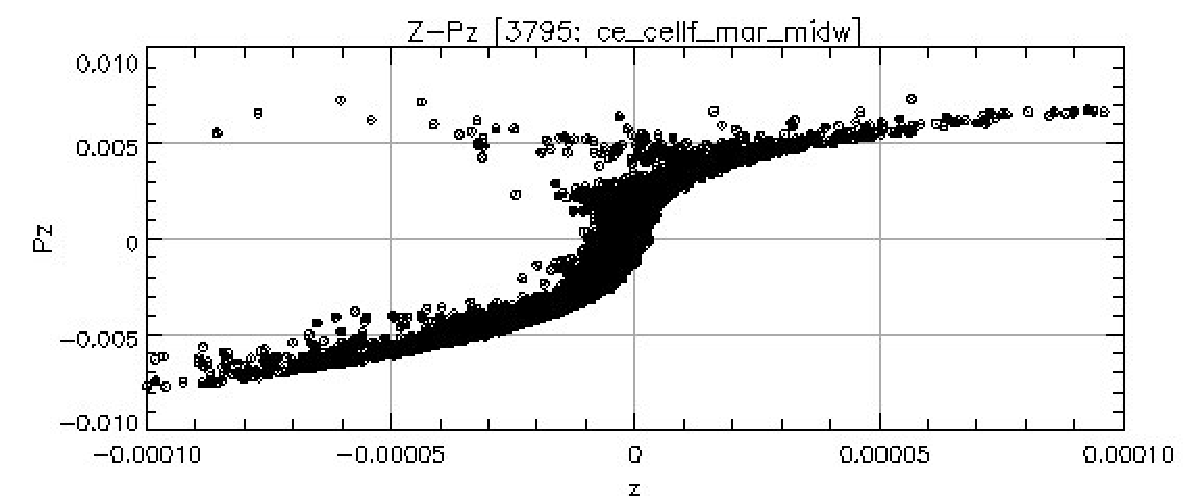
\includegraphics[width=5in]{phase-space.pdf}
  \caption{Example Phase Space plot.}
  \label{f:phase.space}
\end{figure}

A \vn{phase space} plot displays a particle or particles phase space
coordinates at a given location. Phase space plotting is associated
with a \vn{graph} by setting \vn{graph%type} equal to
\vn{"phase_space"}. The concepts here are similar to data plotting
(\sref{s:plot.data}). An example is show in Figure~\ref{f:phase.space}.
Example Phase Space template:
\begin{example}
  &tao_template_plot
    plot%name = "zphase"
    plot%x%min =   -10e-3
    plot%x%max = 10e-3
    plot%x%major_div_nominal = 4
    plot%x%label = "z"
    plot%n_graph = 1
  /

  &tao_template_graph
    graph_index = 1
    graph%name = "z"
    graph%type = "phase_space"
    graph%box = 1, 1, 1, 1
    graph%title = "Z-Pz"
    graph%margin =  0.12, 0.12, 0.12, 0.12, "%BOX"
    graph%y%label = "Pz"
    graph%y%max = 3
    graph%y%min = -3
    graph%y%major_div_nominal = 4
    graph%n_curve = 1
    curve(1)%data_type_x = "z" 
    curve(1)%data_type = "pz" 
    curve(1)%data_source = "beam"
    curve(1)%ele_ref_name = "BEGINNING"
  /
\end{example}

For a \vn{"phase_space"} type graph, \vn{curve%data_type_x} determines
what phase space coordinate is plotted along the x-axis and
\vn{curve%data_type} determines what phase space coordinate is plotted
along the y-axis. The phase space coordinates are:
\index{x}\index{px}\index{y}\index{py}\index{z}\index{pz}
\begin{example}
  "x"
  "px"
  "y"
  "py"
  "z"
  "pz"
  "intensity"       -- Photon total intensity 
  "intensity_x"     -- Photon intensity along x-axis 
  "intensity_y"     -- Photon intensity along y-axis
  "phase_x"         -- Photon phase along x-axis
  "phase_y"         -- Photon phase along y-axis
\end{example}
In this example above, the $x$-axis of the plot will correspond to the
$z$ phase space coordinate and the $pz$-axis will correspond to the
$px$ coordinate.

\index{curve!ele_ref_name}\index{curve!ix_ele_ref}
To change the place in the lattice where the data for the
\vn{phase_space} curve is evaluated, use the \vn{set curve
ele_ref_name} or \vn{set curve ix_ele_ref} commands.

If \vn{graph%type} is \vn{"phase_space"} then \vn{curve%data_source} 
must be either:
\begin{example}
  "beam"
  "multi_turn_orbit"
  "twiss"
\end{example} 
\vn{"beam"} indicates that the points of the phase space plot
will be obtained correspond to the positions of the particles within a
tracked beam. \vn{multi_turn_orbit"} is used for rings where a single
particle is tracked multiple turns and the position of this particle
is recorded each turn. In this case, a \vn{d2_data} structure must
have been set up to hold the turn--by--turn orbit. This \vn{d2_data}
structure must be called \vn{multi_turn_orbit} and must have
\vn{d1_data} data arrays for the phase space planes to be plotted. For
example, if the phase space plot is \vn{x} versus \vn{px}, then there
must be \vn{d1_data} arrays named \vn{"x"} and \vn{"px"}. The number
of turns is determined by the setting of \vn{ix_max_data} in the
\vn{tao_d1_data} namelist (\sref{s:init.data}). Using \vn{"twiss"} as
the \vn{curve%data_source} indicates that the phase space plot will be
an ellipse whose shape is based upon the Twiss and coupling
parameters, and the normal mode emittances. If the normal mode
emittances have not been computed then a nominal value of 1e-6~m-rad
is used.

